\chapter{Data Acquisition, SITS Datasets and Preprocessing}
\label{chapter:meth_data}

This chapter describes the methodology for acquiring, curating, and preprocessing the RS data used in this work, including an overview of the datasets used. The \autoref{sec:data_sources} presents the primary data sources, including plot boundaries and crop reference maps. The \autoref{sec:dataset_creation} details the pipeline developed for creating plot-level crop classification datasets with rigorous filtering. The \autoref{sec:lit_pipe} explores the lightweight strategy for downloading SITS using cloud computing. The \autoref{sec:datasets_overview} details the datasets generated for the Texas, California, and Brazil regions. Finally, the \autoref{sec:agl} presents the open-source AgriGEE.lite library, developed by us to encapsulate the lightweight method among other functions, in order to facilitate the reproducibility of the research or the initiation of others.

\section{Data Sources}\label{sec:data_sources}

The quality and reliability of \ac{ML} models depend primarily on the data sources used. This section details the databases used, addressing their characteristics, authors, resolutions, and specific applications. The \autoref{sec:varda} describes Varda Global FieldID, used for plotting agricultural areas. Subsequently, the \autoref{sec:mapbiomas} and \ref{sec:usda} present, respectively, Mapbiomas Brasil and the USDA Cropland Data Layer, which provide crop classification labels for the agricultural crop classes in the study regions.

\subsection{Varda Global FieldID}
\label{sec:varda}

Varda Global FieldID\footnote{Varda Global FieldID: \url{https://fieldid.varda.ag/hub/downloads}} is an international initiative developed by Varda, whose main objective is to create a standardized and universal system for identifying and tracking agricultural parcels delineations on a global scale (see Figures \ref{fig:varda_ba}, \ref{fig:varda_rs} and \ref{fig:varda_fresno}). This project is a collaborative effort to gather, harmonize, and make available geospatial information on agricultural parcels from multiple institutional, governmental, commercial, and community sources, with a unique identifier for each cultivated area. 

\begin{figure}[!ht]
    \centering
    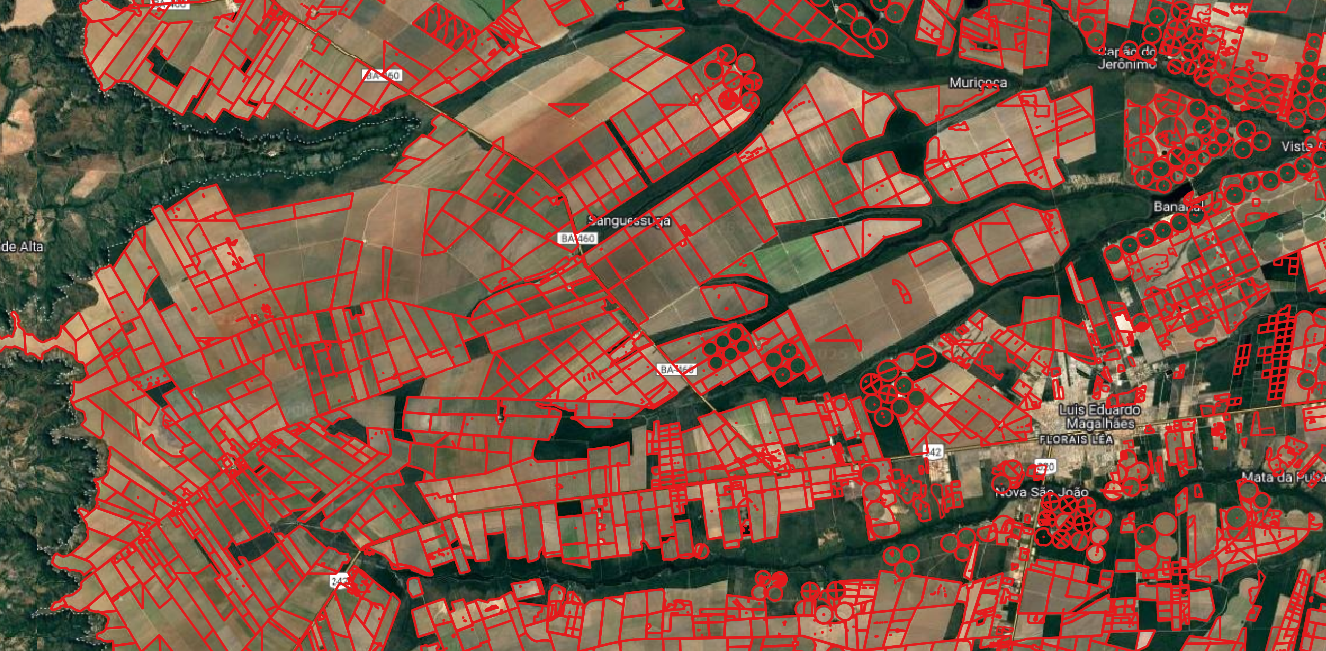
\includegraphics[clip,trim=0.275in 0.55in 0.275in 0.55in,width=1\textwidth]{figures/6_methodology/varda/varda_lem.png}
    \caption{VARDA plots in the municipality of Luis Eduardo Magalhães, Bahia - Brazil.}
    \label{fig:varda_ba}
    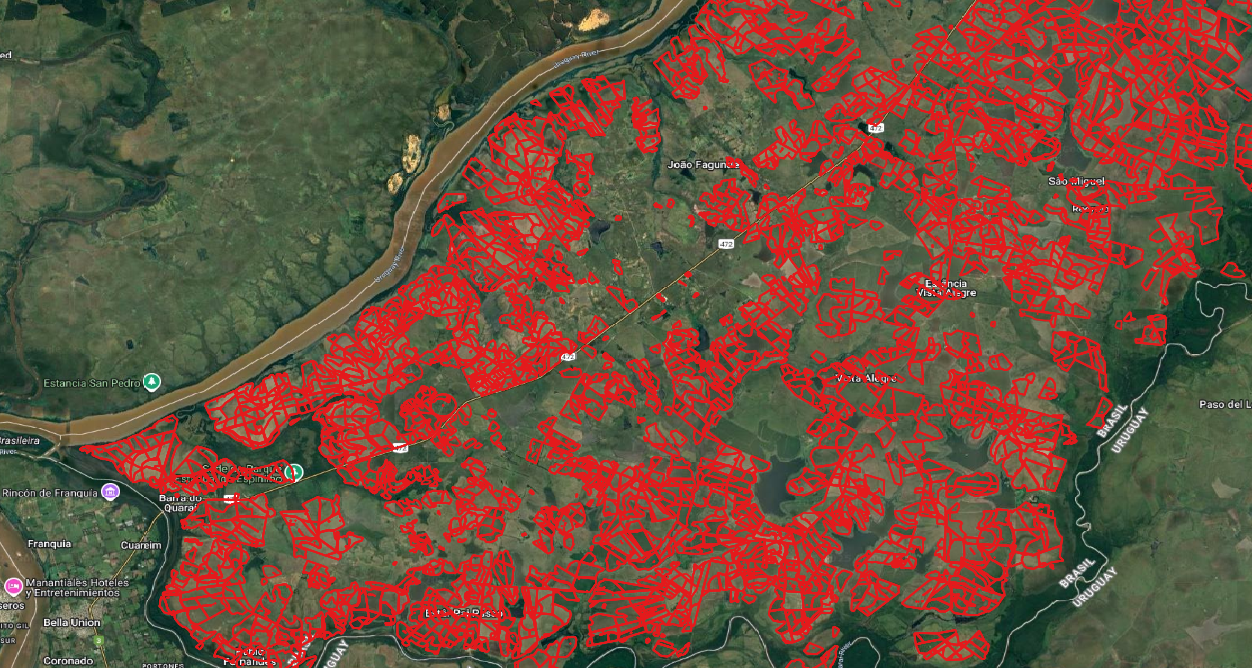
\includegraphics[clip,trim=0.275in 0.55in 0.275in 0.55in,width=1\textwidth]{figures/6_methodology/varda/varda_quarai.png}
    \caption{VARDA plots in the municipality of Barra do Quaraí, Rio Grande do Sul - Brazil.}
    \label{fig:varda_rs}
    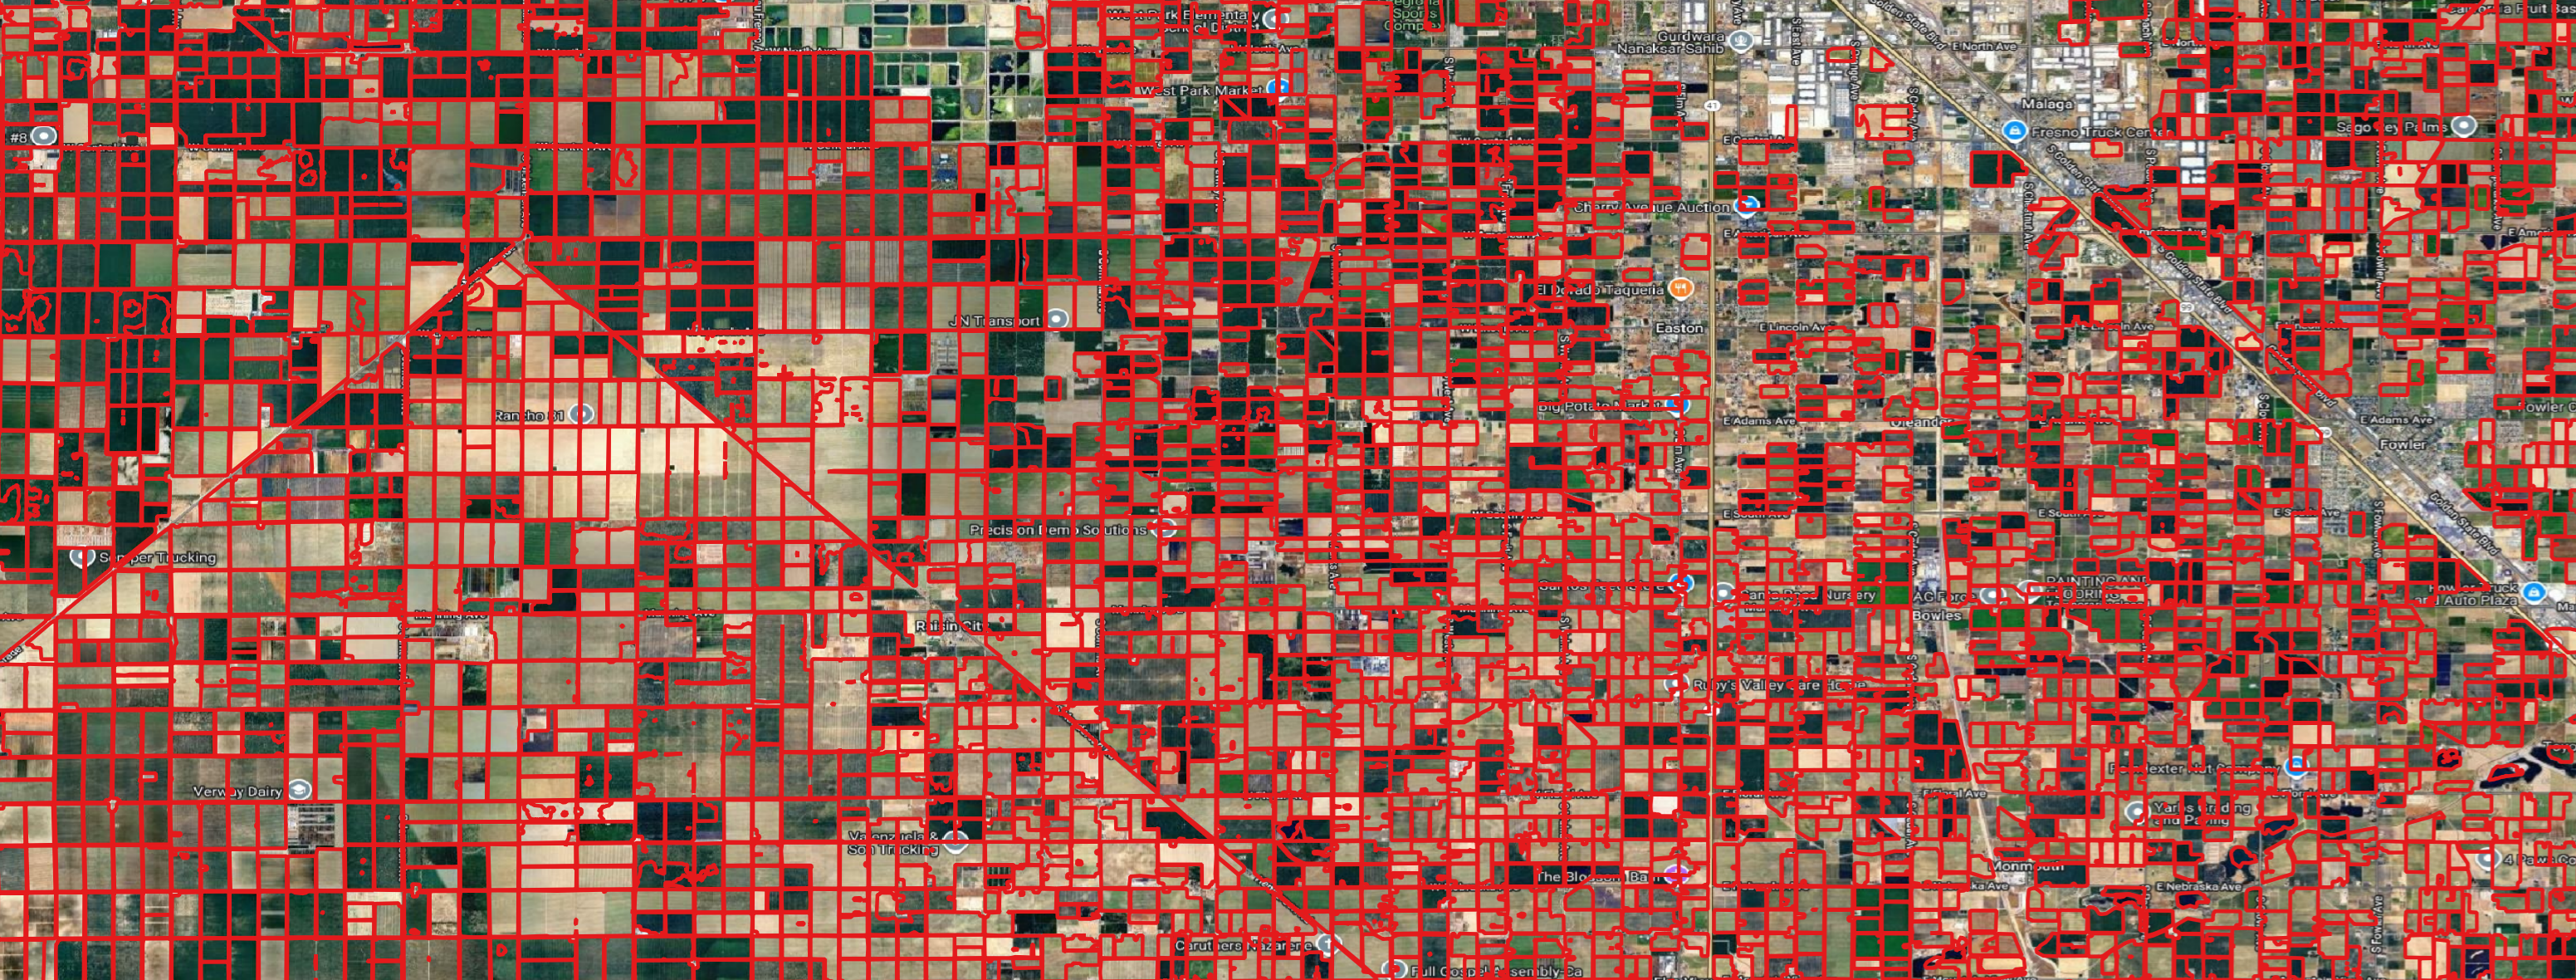
\includegraphics[clip,trim=0.275in 0.55in 0.275in 0.55in,width=1\textwidth]{figures/6_methodology/varda/varda_fresno.png}
    \caption{VARDA plots in the municipality of Fresno, California - USA.}
    \label{fig:varda_fresno}
\end{figure}

The database is updated monthly and contains data from Argentina, Belgium, Brazil, Canada, the Czech Republic, Germany, Denmark, Spain, Estonia, Finland, France, the United Kingdom, India, Italy, Japan, Lithuania, Latvia, the Netherlands, Norway, Poland, Sweden, the United States, and South Africa. In addition to the monthly files, it is possible to obtain data from APIs, which were not used in this study. It is quite noticeable, due to common errors in convolutional models (see Figure \ref{fig:varda_errors}), that most of the plots were generated using \ac{DL} models with the Sentinel 2 MSI sensor, which has a maximum spatial resolution of 10 meters. Access to Global FieldID is free for consultation and download when used in academic research and non-commercial projects.

\begin{figure}[!ht]
    \centering
    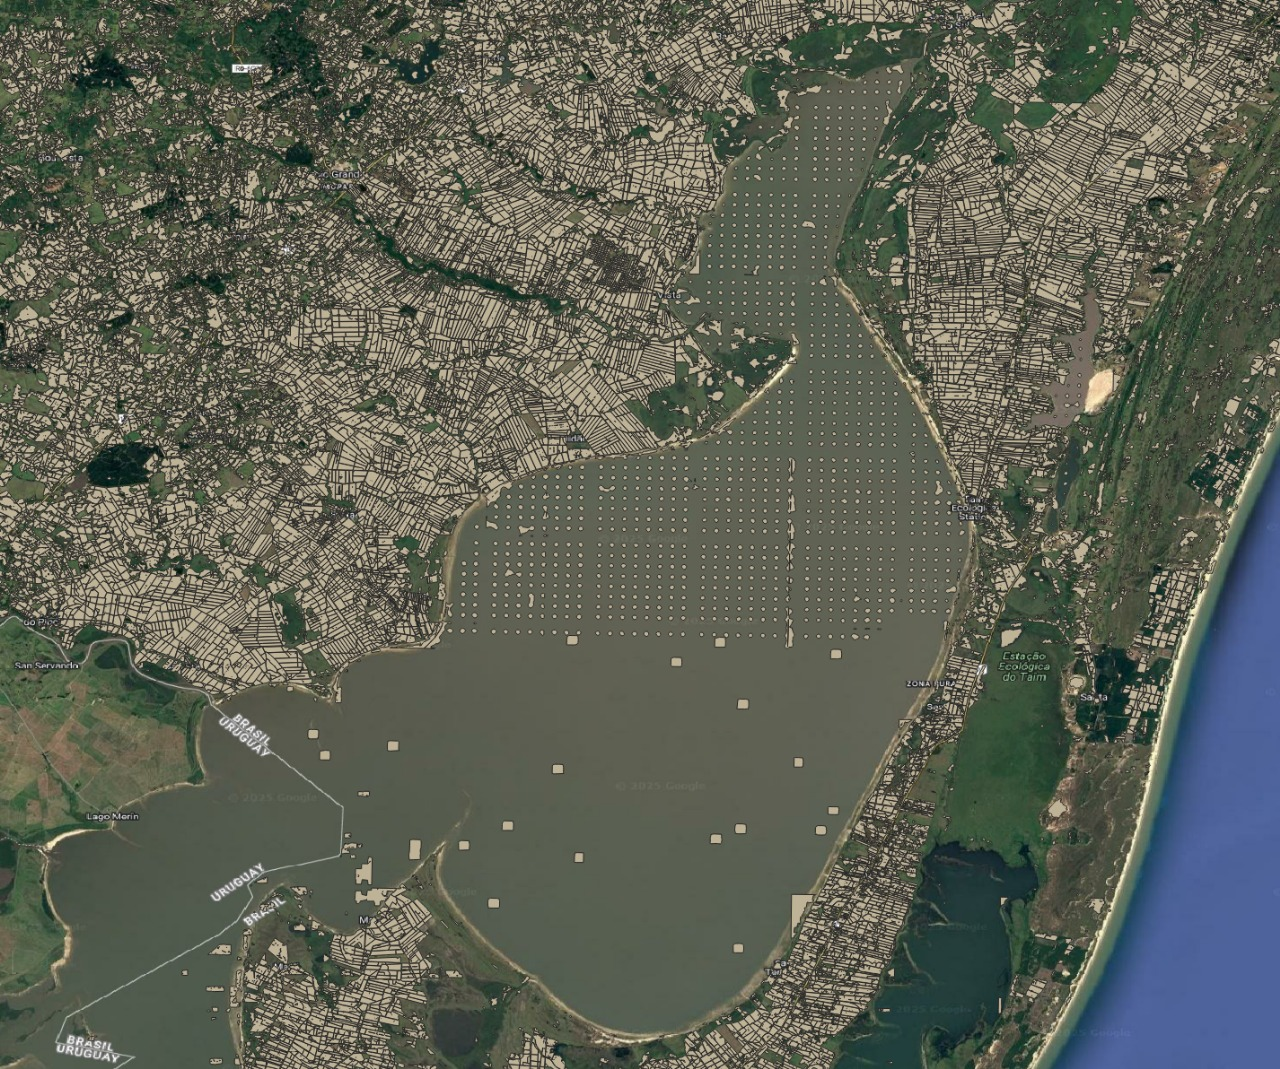
\includegraphics[clip,trim=0.275in 0.55in 0.275in 0.55in,width=1\textwidth]{figures/6_methodology/varda/varda_erros.jpg}
    % }
    \caption{Agricultural plots mistakenly identified in the water in Lagoa dos Patos, in the extreme south of Brazil, on the border between Brazil and Uruguay.}
    \label{fig:varda_errors}
\end{figure}

Parcels smaller than 1 hectare were filtered out, as they are practically just noise in the VARDA dataset. In addition, it is noteworthy that there are many missing parcels, i.e., parcels that exist in reality but are not present in the dataset - especially in regions where parcels are not so well delimited, such as in southern Brazil.

In terms of data quantity, the VARDA dataset is well spread geographically. For Brazil, there is more data for the southeast region and Bahia, but this is in line with the expected number of agricultural parcels across the country (see Figure \ref{fig:varda_qnt}). In California, there are 277,634 parcels, and in Texas, there are 658,018 parcels - all after filtering out parcels smaller than 1 hectare. The main use of Varda Global FieldID in this work is to delineate each agricultural plot geometry, since the databases with agricultural labels (explained below) do not present such information, and may even unify plots that contain the same crop class, for example.

\begin{figure}[!ht]
    \centering
    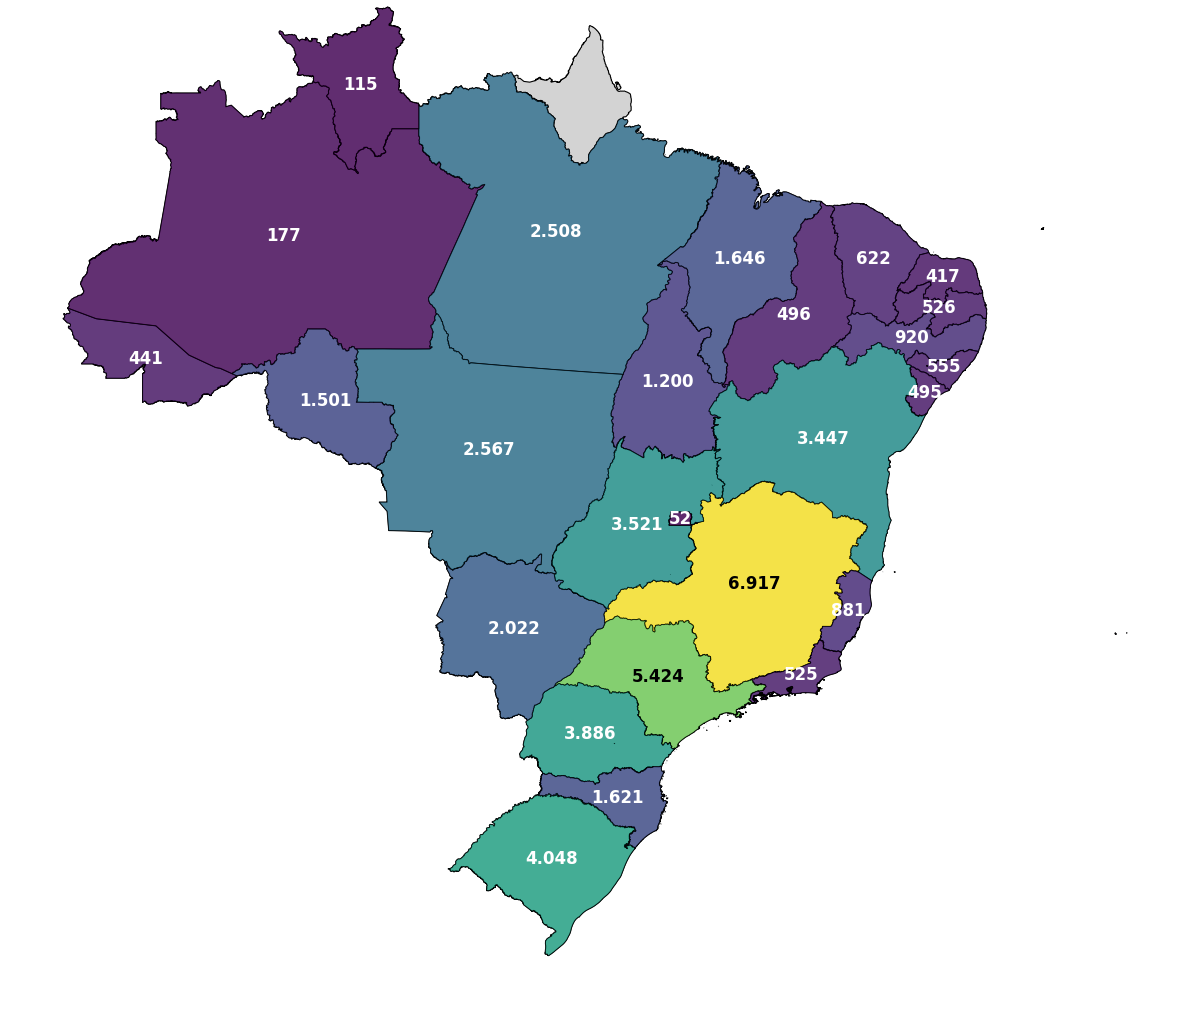
\includegraphics[clip,trim=0.275in 0.55in 0.275in 0.55in,width=0.7\textwidth]{figures/6_methodology/varda/varda_samples_per_uf.png}
    \caption{Number of VARDA parcels in thousands per state in Brazil.}
    \label{fig:varda_qnt}
\end{figure}

\subsection{Mapbiomas Brazil}
\label{sec:mapbiomas}

MapBiomas Brazil \citep{souza2017mapbiomas} is a multi-institutional initiative launched in 2015 by universities, NGOs, and technology companies with the goal of producing annual maps of \ac{LULC} in Brazil at a spatial resolution of 30 meters, covering the historical series from 1985 to the present. The project is organized by biomes (Amazon, Atlantic Forest, Caatinga, Cerrado, Pampa, and Pantanal) and by cross-cutting themes, including Agriculture, Pasture, Forestry, Mining, Coastal Zone, and Urban Area. The methodology is based on the classification of annual mosaics of Landsat images (TM, ETM+, OLI-TIRS sensors), processed on the Google Earth Engine platform. The images undergo cloud/shadow removal and temporal composition optimized for each biome and cross-cutting theme, aiming to maximize spectral contrast between classes. Classification is performed mainly by Random Forest algorithms, one for each year and biome/theme, with training samples collected mainly from stable areas between 1985-2022. For specific agricultural classes and other specific uses, U-Net is also employed.

In the cross-cutting theme of Agriculture, the MapBiomas methodology subdivides the class into temporary and perennial crops, distinguishing up to ten agricultural classes, which are: Citrus, Coffee, Forest Plantation, Palm Oil, Pasture, Other Perennial Crops, Rice, Soybean, Sugar Cane, and Other Temporary Crops (see Figure \ref{fig:mapbiomas}). The detection of these crops involves the use of temporal mosaics per scene, allowing characteristic phenological patterns to be captured.

\begin{figure}[!ht]
    \centering
    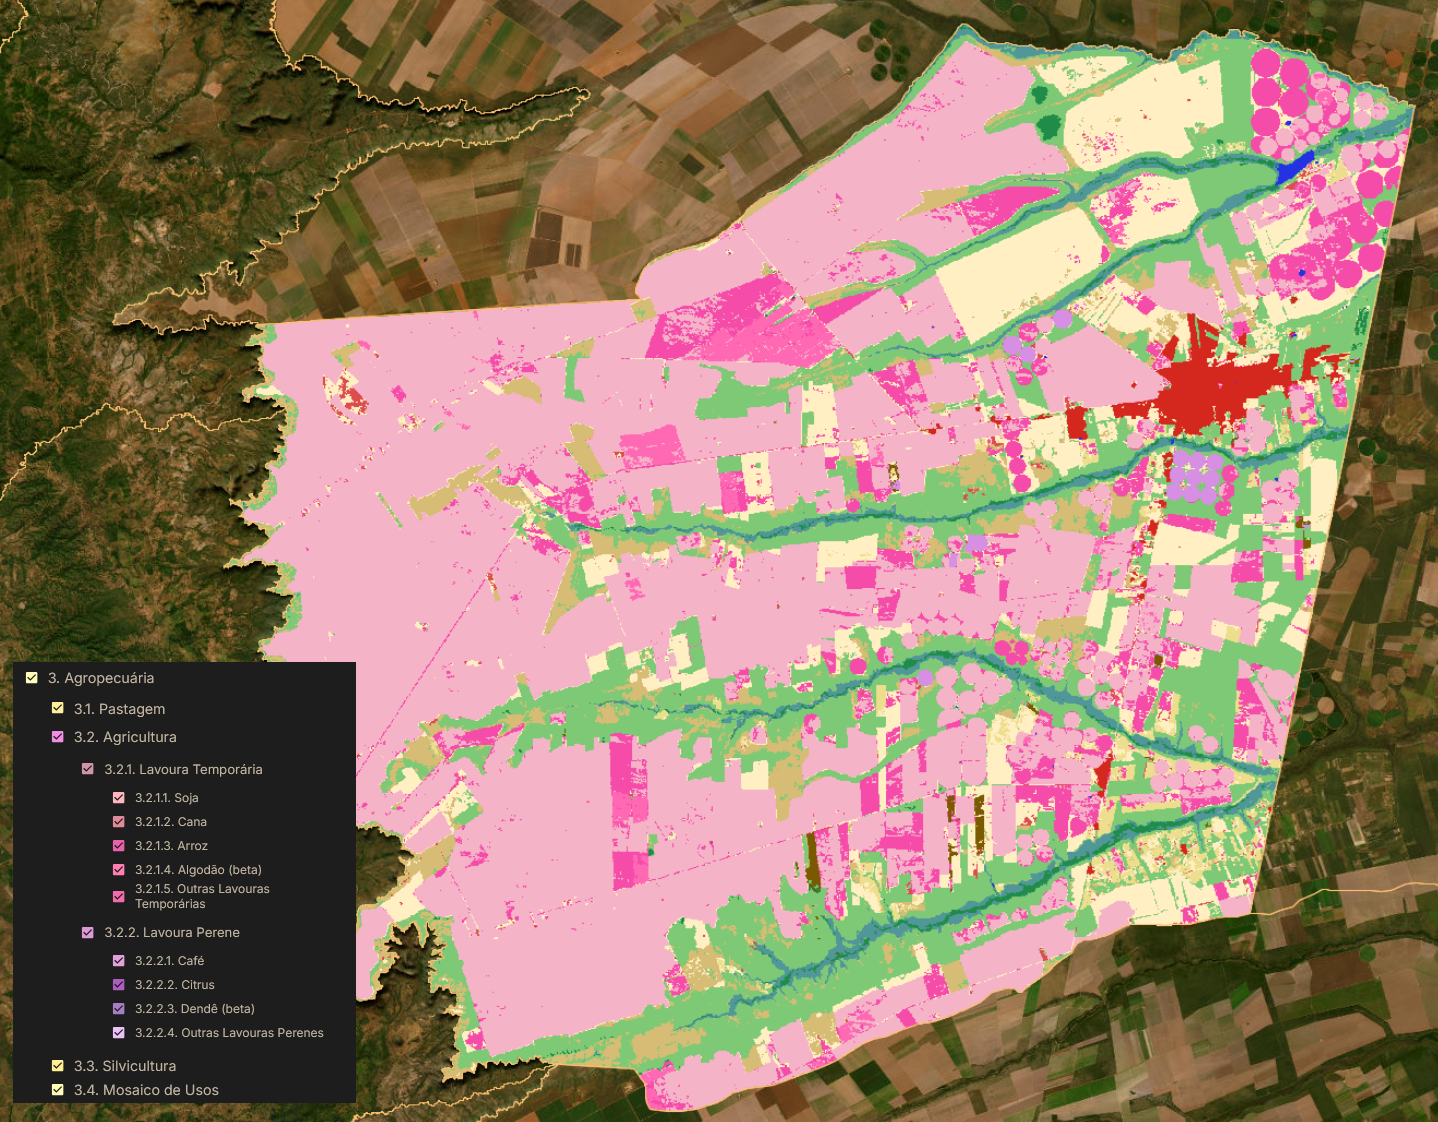
\includegraphics[width=.95\textwidth]{figures/6_methodology/mapbiomas.png}
    \caption{The Mapbiomas 2023 Cropland Raster classification for the city of Luís Eduardo Magalhães, Bahia.}
    \label{fig:mapbiomas}
\end{figure}

Spatial and temporal filters are applied in post-processing to remove noise, correct unrealistic transitions, and stabilize time series. The rules of prevalence between biomes and themes ensure consistency in map integrations. The accuracy assessment of Collection 9 was conducted with approximately 85,000 independent samples per year, for the entire national territory, from 1985 to 2022. Of these, about 10,000 were used for training in the Amazon biome. The validation set, with approximately 75,000 samples/year, was labeled by experts via visual interpretation of Landsat images, MODIS-NDVI series, and high-resolution images. The average overall accuracy for Level 2 of the legend- which contains the classes used for agriculture - was 89.8\%.

However, some details of the Mapbiomas data used in this study are important to highlight. First, Mapbiomas is very clear that its data is LULC and not agricultural land use, which implies that areas classified as agricultural may not actually be in active agricultural use, i.e., an area of temporary crops may mean that temporary crops are normally planted there, but in that specific year it may be fallow or planted with another crop not included in the classification. Therefore, some confusion between certain crops is to be expected, for example between sugarcane and soybeans, as soybean planting is used to regenerate the soil before planting sugarcane, which is a very common crop rotation in Brazil.

The primary use of Mapbiomas Brasil in this work is to extract the labels of the crop classes present in the country. Note that there are other sources of crop class data for Brazil, notably the CONAB maps\footnote{Conab (Companhia Nacional de Abastecimento): \url{https://portaldeinformacoes.conab.gov.br/mapeamentos-agricolas.html}}, but Mapbiomas Brasil, as far as we researched, is the only source with a single map that covers the entire country containing all the main agricultural crops.

\subsection{USDA Cropland Raster}
\label{sec:usda}

The Cropland Data Layer (CDL) is an annual, georeferenced raster product specific to agricultural crops produced by the National Agricultural Statistics Service (NASS) of the \ac{USDA} (see Figure \ref{fig:usda}). The program, which began in 1997 and expanded its coverage to the entire continental United States in 2008, uses satellite imagery and ground truth data to map agricultural land use and cover.

\begin{figure}[!ht]
    \centering
    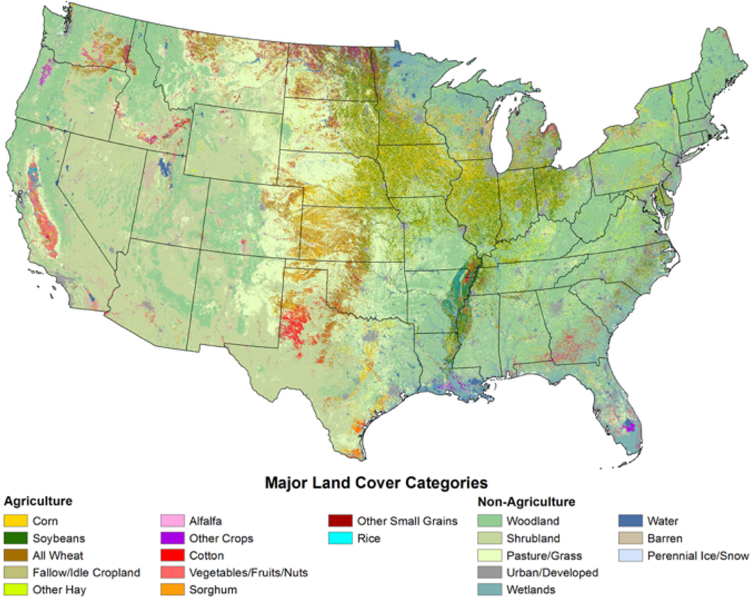
\includegraphics[width=.95\textwidth]{figures/6_methodology/USDA.png}
    \caption{The USDA Cropland Raster.}
    \label{fig:usda}
\end{figure}

Recently, for the 2024 crop year, the program underwent a methodological update, increasing the spatial resolution to 10 meters and migrating the processing flow to the GEE, using \ac{RF}. Previously (2008-2023), the resolution was 30 meters and mostly used \ac{DT}, although we used the 30 meter spatial resolution because we also used data prior to 2023.

The current methodology integrates optical images from OLI/TIRS (Landsat 8 and 9) and MSI (Sentinel-2A and 2B) sensors, harmonized and composited into 10-day medians to reduce cloud cover. In addition to the visible, NIR, SWIR, and RedEdge bands, auxiliary data such as the USGS 3DEP Digital Elevation Model and the official US LULC product, the National Land Cover Database (NLCD), are used.

The strength of the CDL lies in the quality of its training data. For agricultural classes, the model is trained with data from the Farm Service Agency (FSA) Common Land Unit (CLU). The CLU consists of administrative data reported directly by farmers participating in government programs, providing robust and detailed ground truth. For non-agricultural classes, NLCD data is used as a reference. The CDL distinguishes more than 100 land cover categories, focusing on major commodities (such as corn, soybeans, wheat, and cotton) and specialty crops (such as almonds, walnuts, and citrus).

Product accuracy is assessed annually using independent validation sets derived from the FSA CLU. For the 2024 product, producer accuracy for major commodity categories is generally between 85\% and 95\%. The primary use of USDA Cropland Raster in this work is the same as Mapbiomas Brasil, but for US datasets: to remove the labels of the crop classes present in the country.

\section{Pipeline for creating parcel-level crop classification datasets}\label{sec:dataset_creation}

The Figure \ref{fig:meth_datasets} presents the proposed pipeline for creating crop classification datasets at the plot level. The method integrates agricultural plot design data with Cropland Rasters, using Google Earth Engine (GEE) for cloud processing and statistical filtering based on agricultural spectral indices.

\begin{figure}[ht!]
    \centering
    \caption{Graphical abstract showing the pipeline for creating parcel-level crop classification dataset.}
    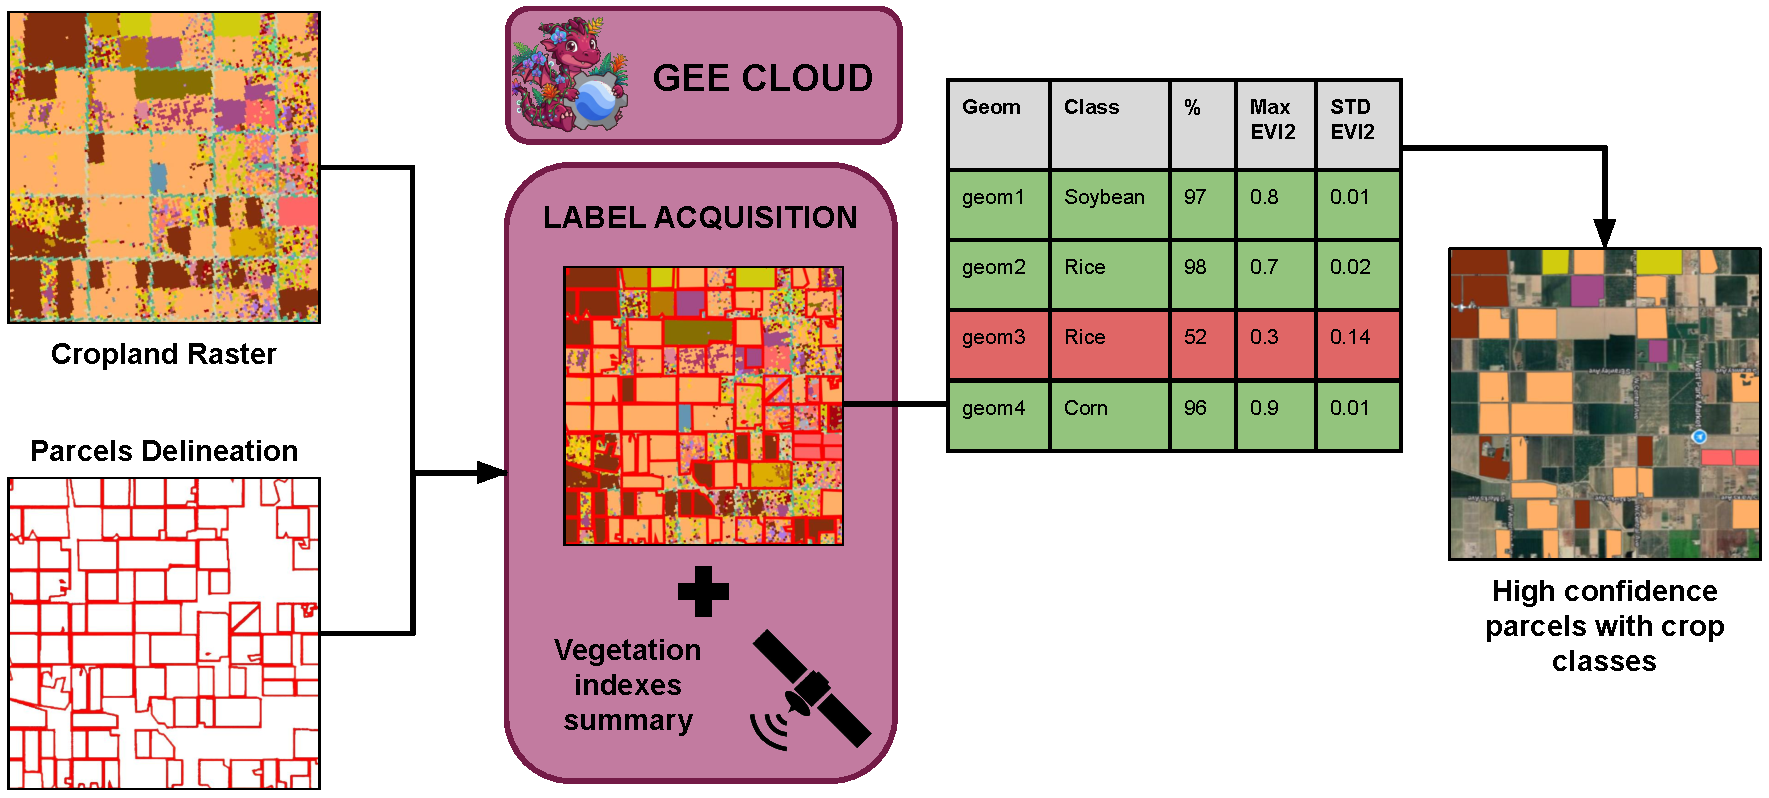
\includegraphics[width=.95\linewidth]{figures/6_methodology/creating_datasets.pdf}
    \label{fig:meth_datasets}
\end{figure}

First, basic descriptive statistics for each geometry are extracted. The crop class of a plot is determined by the most frequent label within that polygon in the corresponding year. To support the subsequent filtering step, the necessary vegetation indices are calculated via GEE Cloud, allowing verification of the plot's agronomic viability.

After that, a filtering step is applied to discard malformed or inconsistent parcels. This process imposes the following exclusion criteria:

\begin{itemize}
\item \textbf{Label Consistency:} It is verified that the dominant crop class in the parcel corresponds to at least 90\% of its pixels. Plots with excessive mixing of classes (as illustrated by \textbf{geom3} in the table in Figure \ref{fig:meth_datasets}) are removed.
\item \textbf{Confidence and Cultivation:} It is ensured that the average confidence of the class pixels is greater than  and that, using the binary cultivation channels, at least 90\% of the pixels are marked as cultivated, if this information exists in the Cropland Raster.
\item \textbf{Agricultural Filter (EVI2):} An agricultural filter was incorporated to eliminate geometries that were not effectively cultivated. Using GEE, the timestamp with the highest \ac{EVI2} is identified, corresponding to the vegetative peak. Samples with a maximum median EVI2 of less than 0.2 or with a spatial standard deviation greater than 0.2 are discarded to remove, respectively, non-agricultural samples or poorly cut parcels.
\end{itemize}

The final result of this pipeline (right side of Figure \ref{fig:meth_datasets}) is a consolidated set of high confidence agricultural parcels, containing only well-delimited geometries with consistent labels, ready for model fine-tuning.

\section{Lightweight SITS download strategy}
\label{sec:lit_pipe}

Figure \ref{fig:meth_download} illustrates the data acquisition flow, designed to operate entirely on Google Earth Engine (GEE) Cloud through the AgriGEE.lite library we developed (which will be better explained in Section \ref{sec:agl}). This approach converts raw and noisy images into treated and statistically representative time series (Treated Resulting \ac{SITS}). The process is divided into four sequential steps described below:

\begin{figure}[ht!]
    \centering
    \caption{Graphical abstract showing the Lightweight SITS download strategy.}
    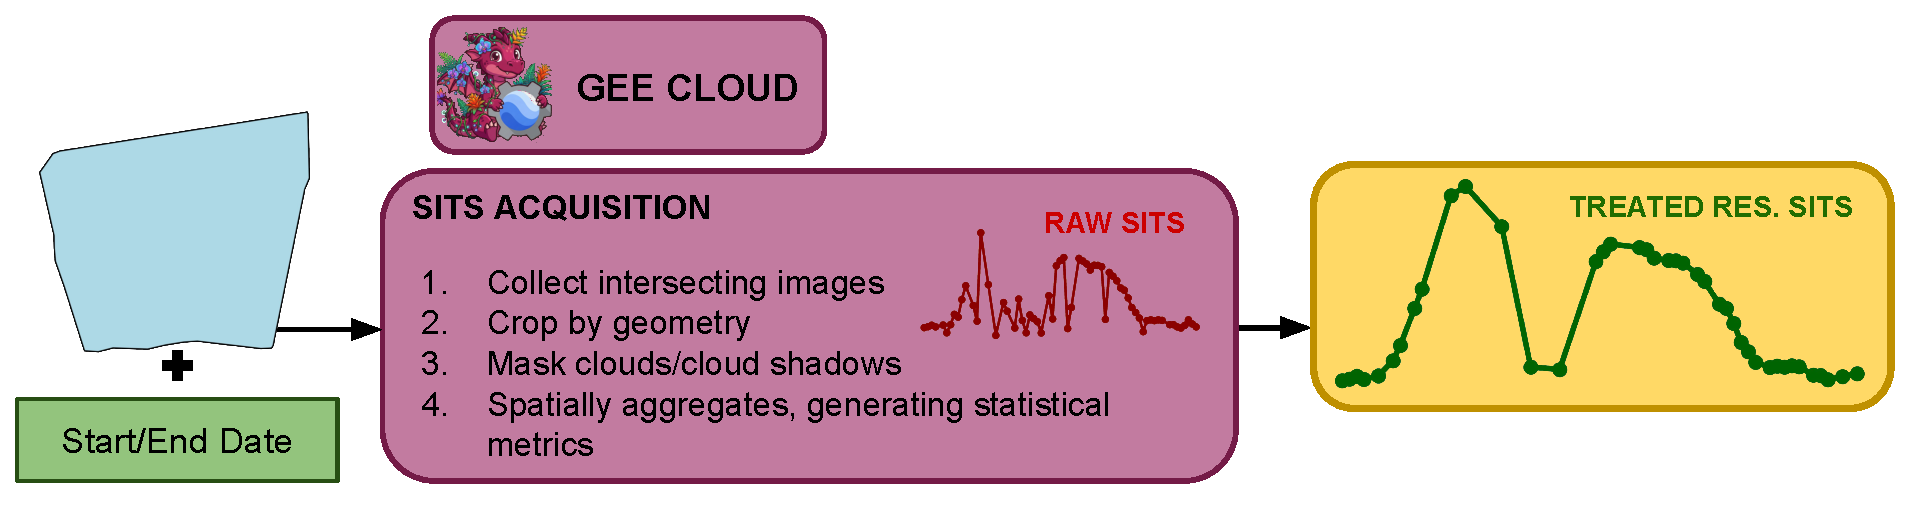
\includegraphics[width=.95\linewidth]{figures/6_methodology/ligthweight_dowload.pdf}
    \label{fig:meth_download}
\end{figure}

\textbf{1. Collect intersecting images} The first step consists of consulting the satellite image catalog, using the corresponding start and end dates. Although the methodology is sensor-agnostic, this work uses Sentinel-2 surface reflectance data, collecting all available scenes that spatially intersect the input geometry.

\textbf{2. Crop by geometry} To ensure that only the area of interest is processed, the collected images are clipped using the parcel outline. 

\textbf{3. Mask clouds/cloud shadows} The third step applies a quality filter. For Sentinel 2, the Cloud Score+ S2 mask is used to remove pixels with a cloud probability greater than 70\%. The pipeline preserves a timestamp as long as at least 20 pixels remain free of clouds or shadows in the parcel. This maximizes the temporal density of the series, recovering information on partially cloudy dates.

\textbf{4. Spatially aggregates, generating statistical metrics} Finally, the pipeline performs spatial aggregation of the remaining valid pixels. For each date, up to 1,000 pixels are randomly sampled within the cropped geometry, and statistics for each spectral band are calculated; in this study, only the median is used. The choice of the median, rather than the mean, aims to mitigate the influence of extreme residual values coming from flaws in the cloud mask. Furthermore, it is important to note that agriculture tends to be uniform within the plot. The result is a lightweight time series, composed of a pseudo-pixel with a single representative value per band per date, drastically reducing the dimensionality of the data while preserving the phenological spectral signature of the crop.

\section{Texas, California and Brazil datasets}
\label{sec:datasets_overview}

To validate the proposed methodology, three distinct datasets based on \ac{SITS} were developed, covering the entire Brazilian territory and the states of California and Texas in the United States. The Brazilian dataset used  Mapbiomas Brasil rasters for class labels (see Section \ref{sec:mapbiomas}), while the datasets for California and Texas used \ac{USDA} cropland data (see Section \ref{sec:usda}). In all scenarios, the definition of agricultural parcels geometries utilized the parcel delineation from Varda Global FieldID (see Section \ref{sec:varda}). The samples consist of the median of the 10 spectral bands of the Sentinel-2/MSI sensor, processed with the Google Cloud Score+\footnote{Google Cloud Score+: \url{https://developers.google.com/earth-engine/datasets/catalog/GOOGLE_CLOUD_SCORE_PLUS_V1_S2_HARMONIZED}} mask to remove clouds and cloud shadows, ensuring the medians only used spectral information from the crops. The US datasets have been previously introduced by us \citep{pintodasilva2025lightweight}, whereas the Brazilian dataset is a new contribution of this work. However, it is imperative to highlight that the creation and public release of the Texas and California datasets stand as a major standalone contribution of this research to the global remote sensing community. By providing highly curated, parcel-level \ac{SITS} benchmarks for prominent North American agricultural regions, these datasets establish a reliable and open-access foundation for evaluating machine learning models under distinct climatic and phenological conditions. Their publication not only ensures the reproducibility of the proposed pipeline but also actively encourages future studies in domain adaptation, transfer learning, and scalable crop monitoring across diverse geographical contexts.

In terms of temporal coverage and design, the datasets reflect the specific agricultural calendars of their respective regions. The Brazilian dataset covers the years 2022 and 2023, using the local agricultural calendar which begins on October 1 and ends on September 30, with parcel geometries dated January 2025. Conversely, the data from California and Texas span from 2019 to 2023 and follow the calendar year (January 1 to December 31), using parcel geometries from July 2024. The selection of these specific dates for the geometries was strategic, targeting the month corresponding to the predominant vegetative peak in each region to improve edge accuracy. Also, it is important to mention that the historical plot delineations are not maintained by the Varda Global Field ID, or that they prevent geometries from each year from being used.

Although class imbalance is very common in agricultural machine learning and exists in all three datasets, the specific class distributions vary significantly. Figures \ref{fig:bar_brazil}, \ref{fig:bar_california}, and \ref{fig:bar_texas} illustrate the crop counts for Brazil, California, and Texas, respectively. In the Brazilian dataset, it is noteworthy that the most common class is Pasture, with almost twice as many classes as the second largest class, Other Temporary Crops. Furthermore, another notable difficulty is that Pasture, Other Temporary Crops, and Other Perennial Crops are classes that contain more than one Crop Type each, making these classes particularly difficult and possibly noisier. Additionally, because Soybeans and Rice are perennial Crop Classes, some confusion with Other Temporary Crops is expected, while Citrus and Palm Oil are likely to be confused with Other Perennial Crops for the same reason.

\begin{figure}[ht!]
    \centering
    \caption{Crop classes distribution in Brazil SITS dataset.}
    \label{fig:bar_brazil}
    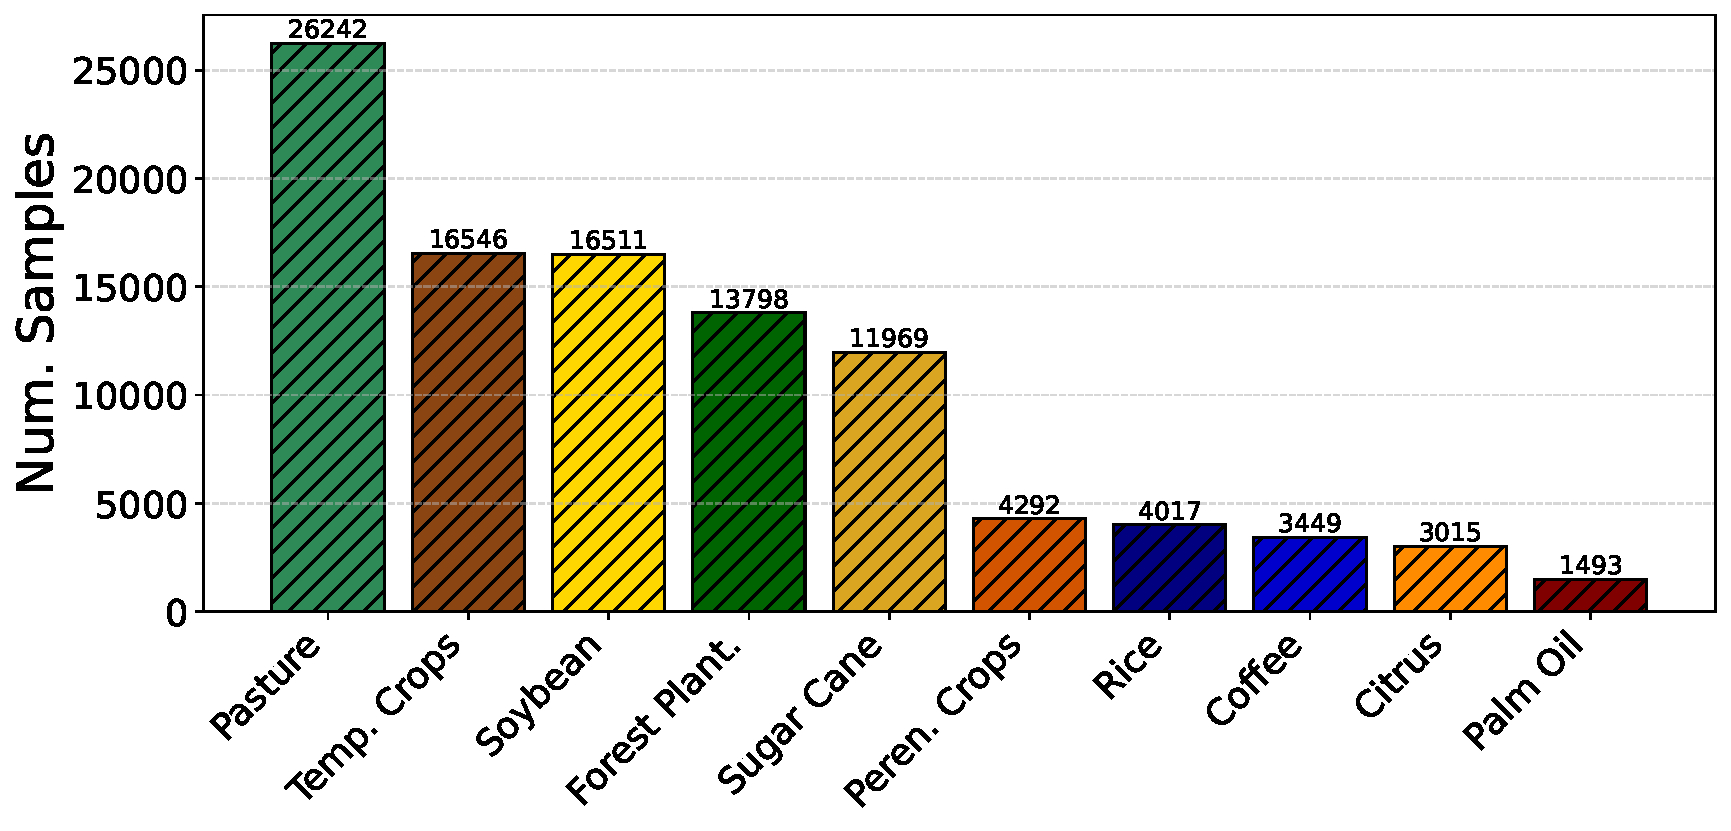
\includegraphics[width=0.6\linewidth]{figures/6_methodology/datasets/brazil_bar_crop.pdf}
\end{figure}

\begin{figure}[ht!]
    \centering
    \caption{Crop classes distribution in California SITS dataset.}
    \label{fig:bar_california}
    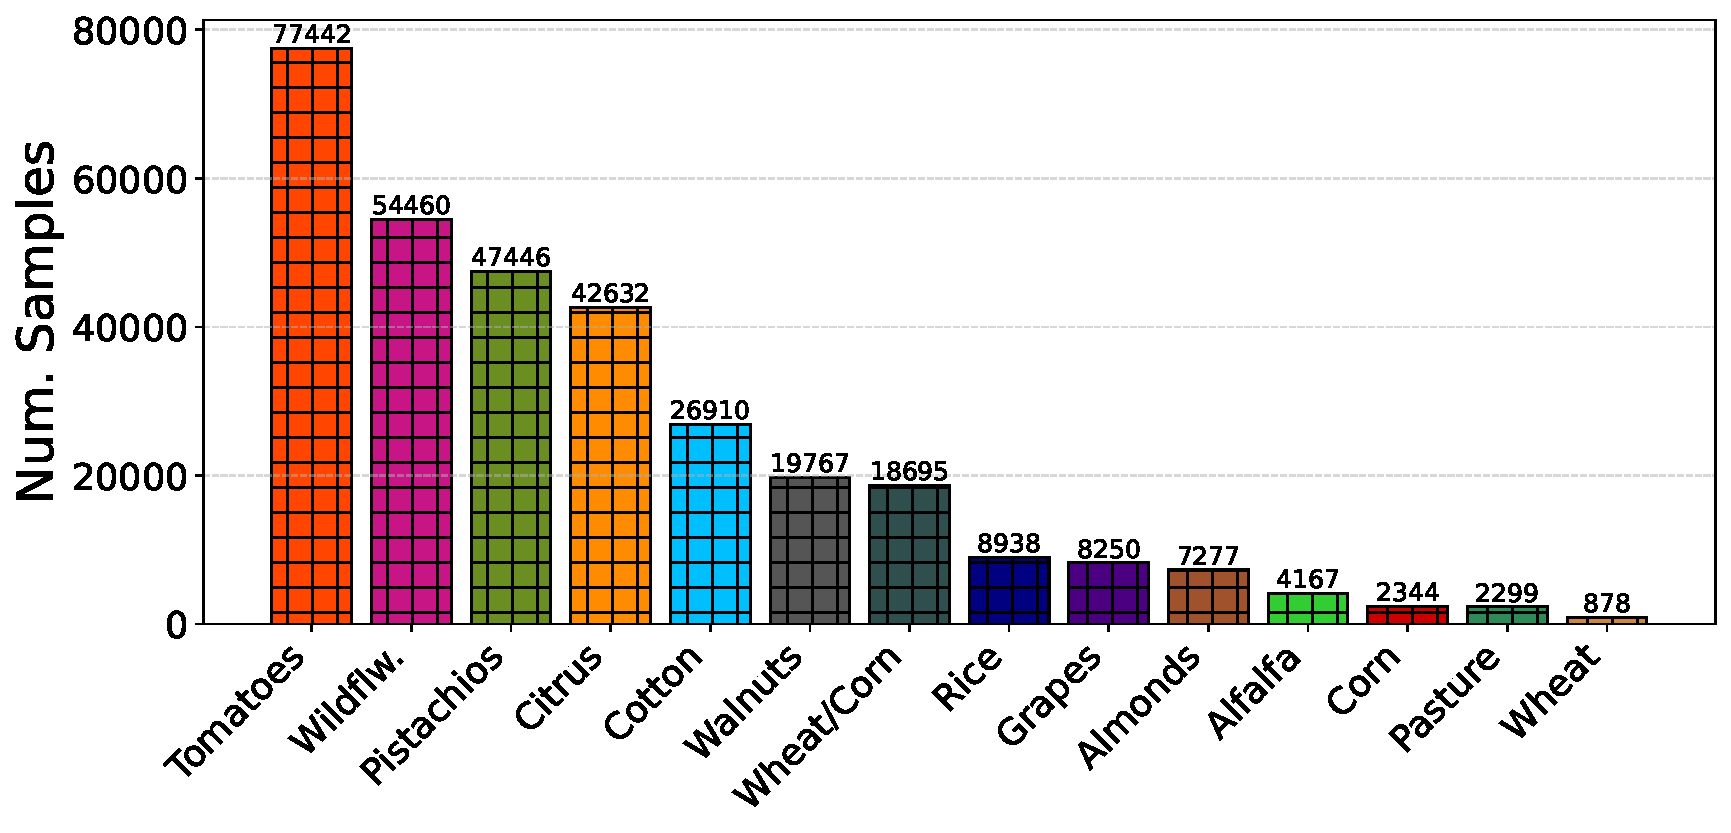
\includegraphics[width=0.6\linewidth]{figures/6_methodology/datasets/california_bar_crop.pdf}
\end{figure}

\begin{figure}[ht!]
    \centering
    \caption{Crop classes distribution in Texas SITS dataset.}
    \label{fig:bar_texas}
        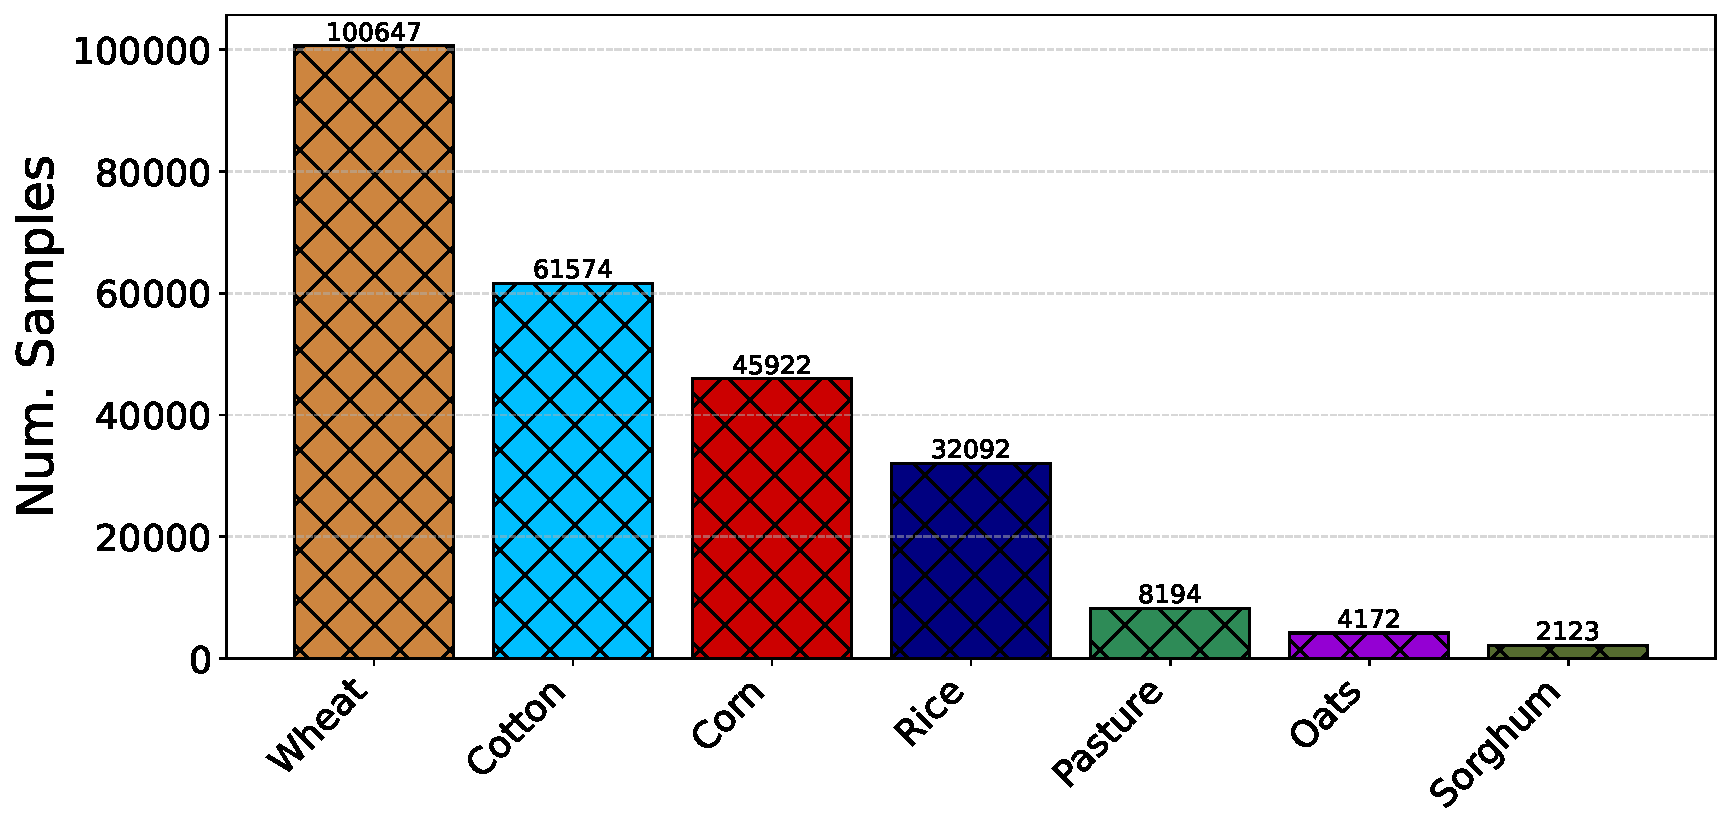
\includegraphics[width=0.6\linewidth]{figures/6_methodology/datasets/texas_bar_crop.pdf}
\end{figure}

Despite the shared challenge of imbalance, the Brazilian dataset is notably more complex than those from California and Texas due to its subcontinental scope and high agricultural variability. As shown in Figure \ref{fig:map_brazil}, the geographical spacing in Brazil leads to distinct regional patterns. For instance, \textit{Soybean} cultivation is heavily concentrated in the Center-West and South, yet planting schedules differ; harvests in the South are generally earlier due to the climate. Other crops, such as \textit{Coffee} and \textit{Sugar Cane}, are clustered in the Southeast, reflecting specific soil and altitude requirements. This heterogeneity requires the model to generalize class features across vastly different biomes. Furthermore, palm oil cultivation is quite geographically localized, as it is planted in degraded areas of the Amazon rainforest. Although the dataset contains plot designs and, consequently, geographic information, this will not be used by the models.

\begin{figure}[ht!]
\centering
\caption{Crop classes regional distribution in Brazil SITS dataset.}
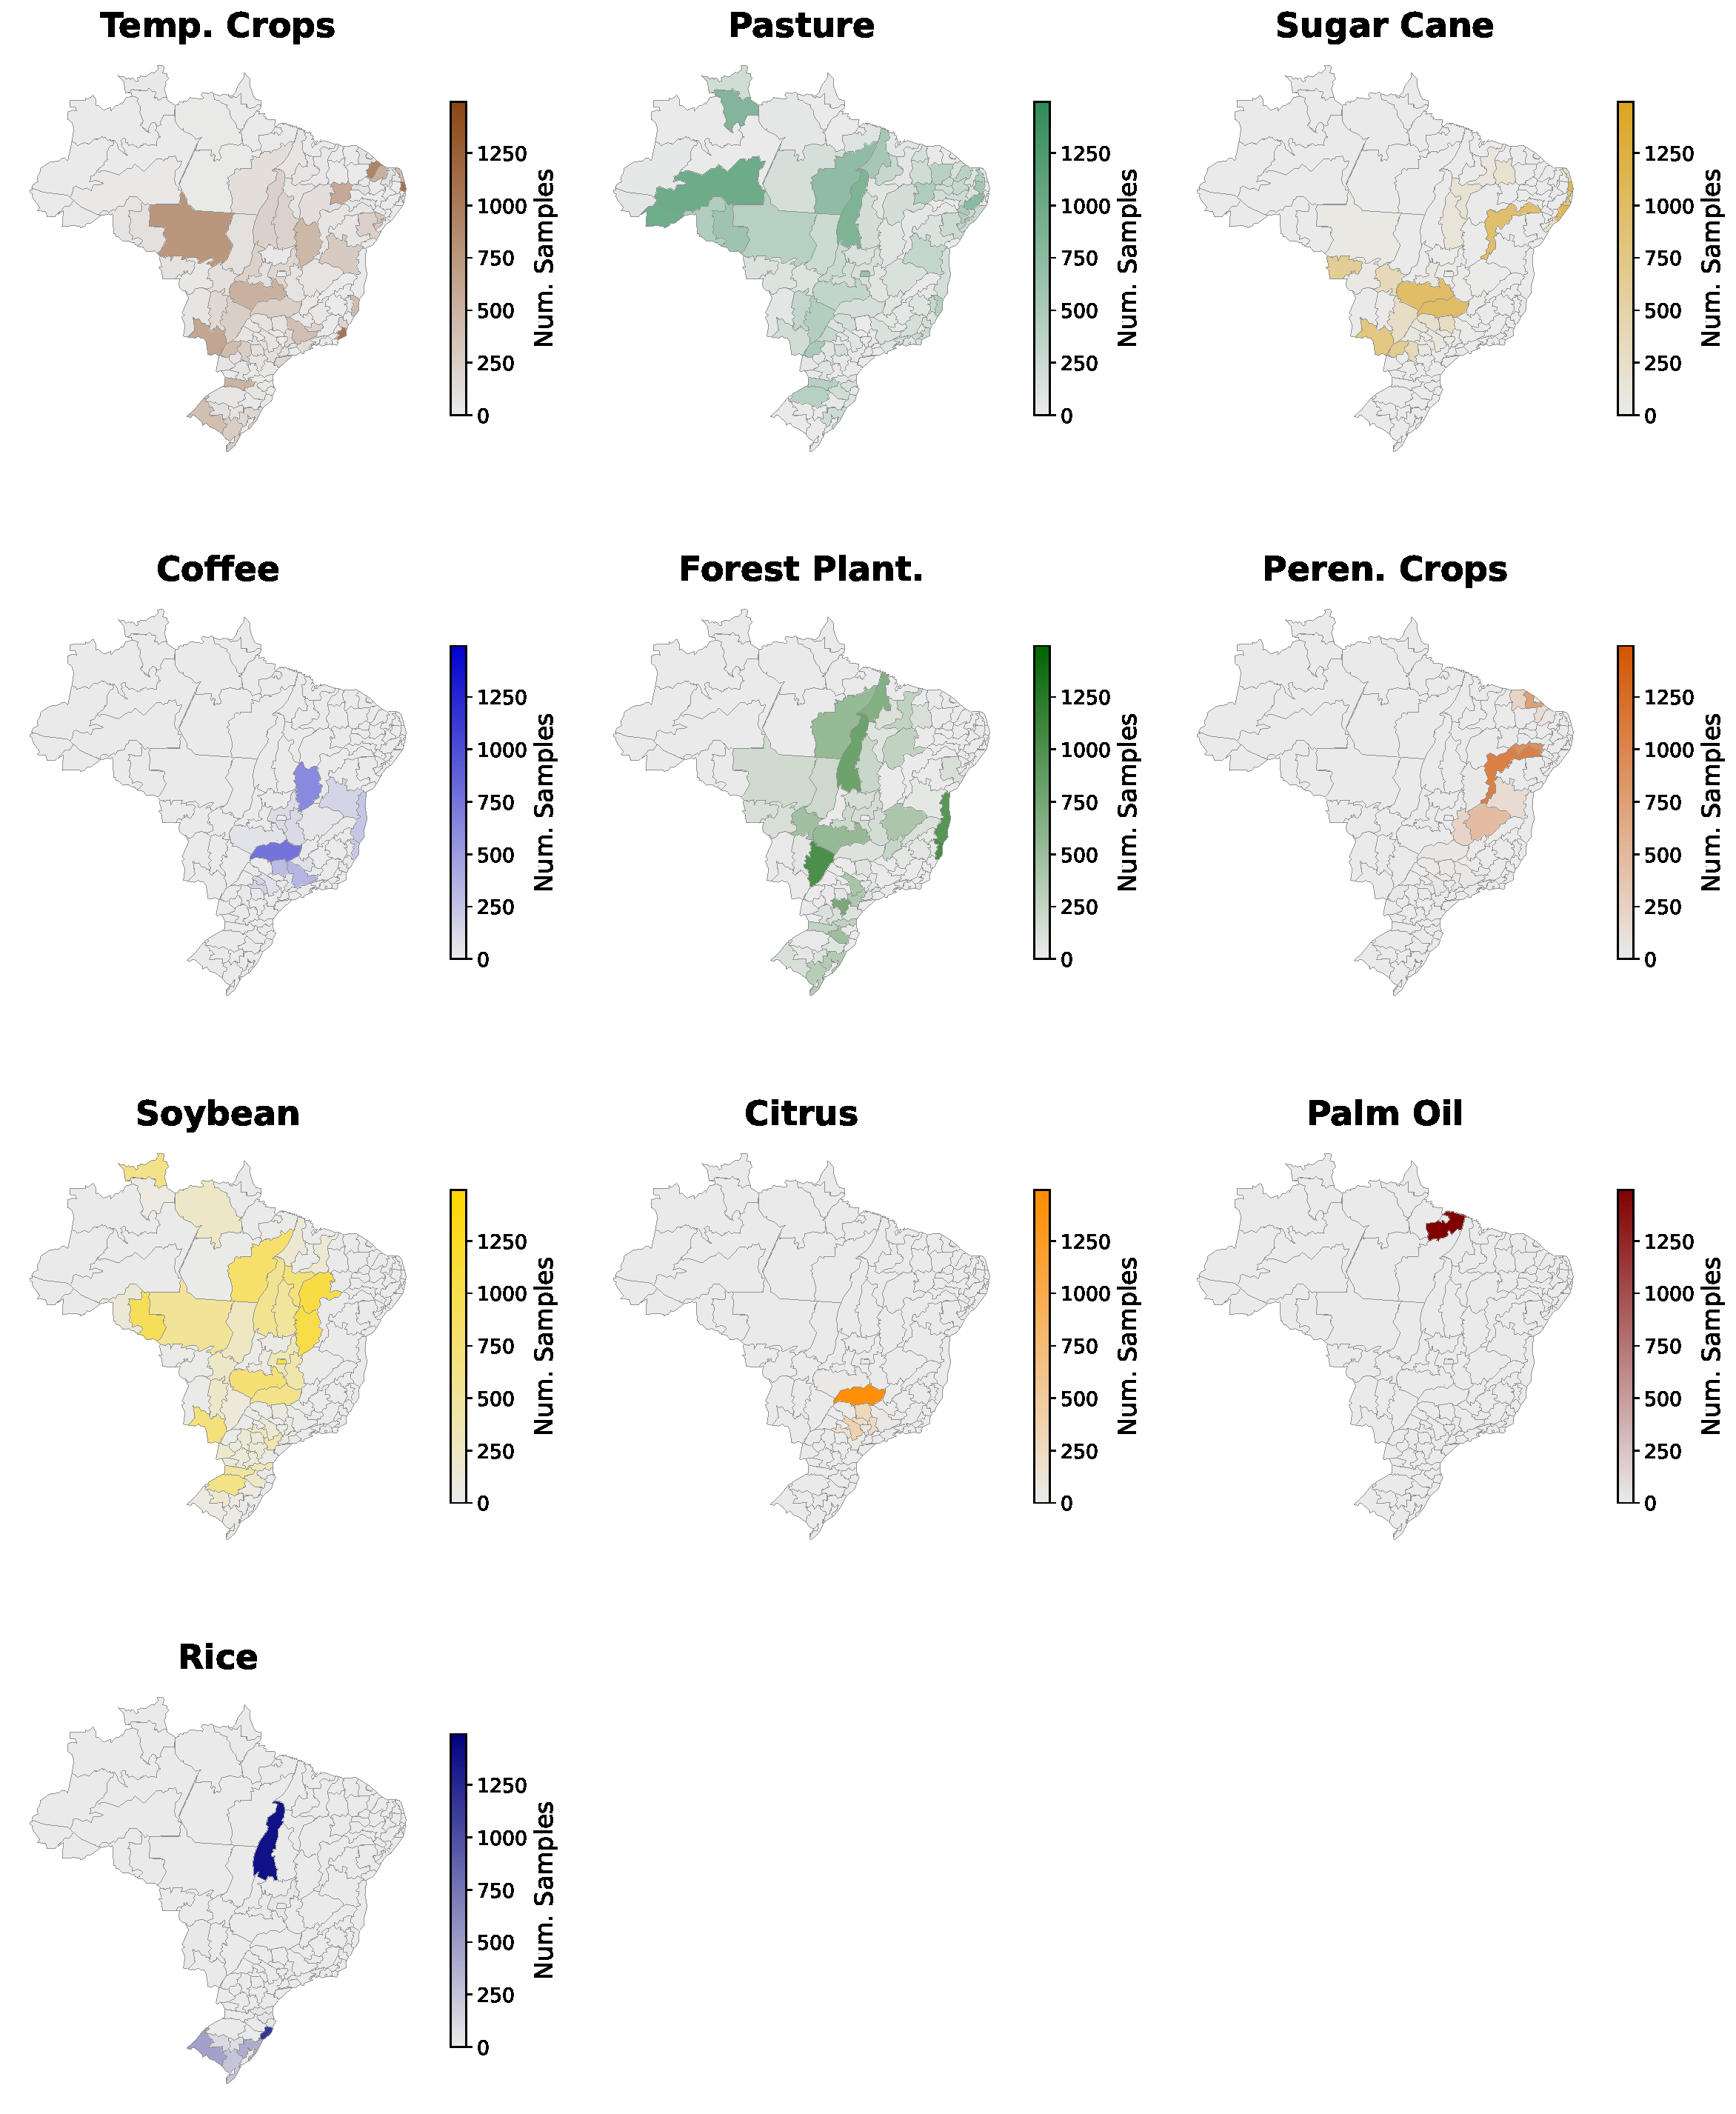
\includegraphics[height=0.7\textheight, keepaspectratio]{figures/6_methodology/datasets/brazil_map_crops.pdf}
\label{fig:map_brazil}
\end{figure}

Furthermore, the phenological behavior of crops in Brazil differs markedly from the US regions. The practice of double cropping (and occasionally triple cropping) in temporary crops is widespread in Brazil. In contrast, agriculture in the US datasets is predominantly single-cycle, with the notable exception of the Wheat/Corn rotation in California. 

This multi-cycle characteristic introduces a specific challenge in the Brazilian dataset: Mapbiomas only provides labels for the primary crop of the year. Consequently, the spectral signals of subsequent crops (often referred to as ``safrinha'') act as noise. This is evident in Figure \ref{fig:evi2_brazil}, where the \textit{Soybean} class exhibits a primary harvest peak followed by secondary EVI2 elevations, likely indicating unregistered corn or cotton. Perennial crops in Brazil, such as \textit{Forest Plantation} and \textit{Citrus}, show stable high EVI2 values, which the model must differentiate from the dynamic peaks of annual crops.

Comparing this to the US datasets, Figure \ref{fig:evi2_california} for California shows the distinct double-peak signature of the labeled \textit{Wheat/Corn} class, while Figure \ref{fig:evi2_texas} for Texas displays clear, single-peak curves for monocultures like \textit{Cotton}, separated by long fallow periods. Furthermore, it is quite evident that the spectral behavior of the crops in both US datasets is much more pronounced and visible in the plots shown, which reinforces that the Brazilian dataset is considerably noisier, inheriting noise from the Mapbiomas Brasil used as a cropland raster.

\begin{figure}[ht!]
\centering
\caption{EVI2 per crop class in Brazil SITS dataset.}
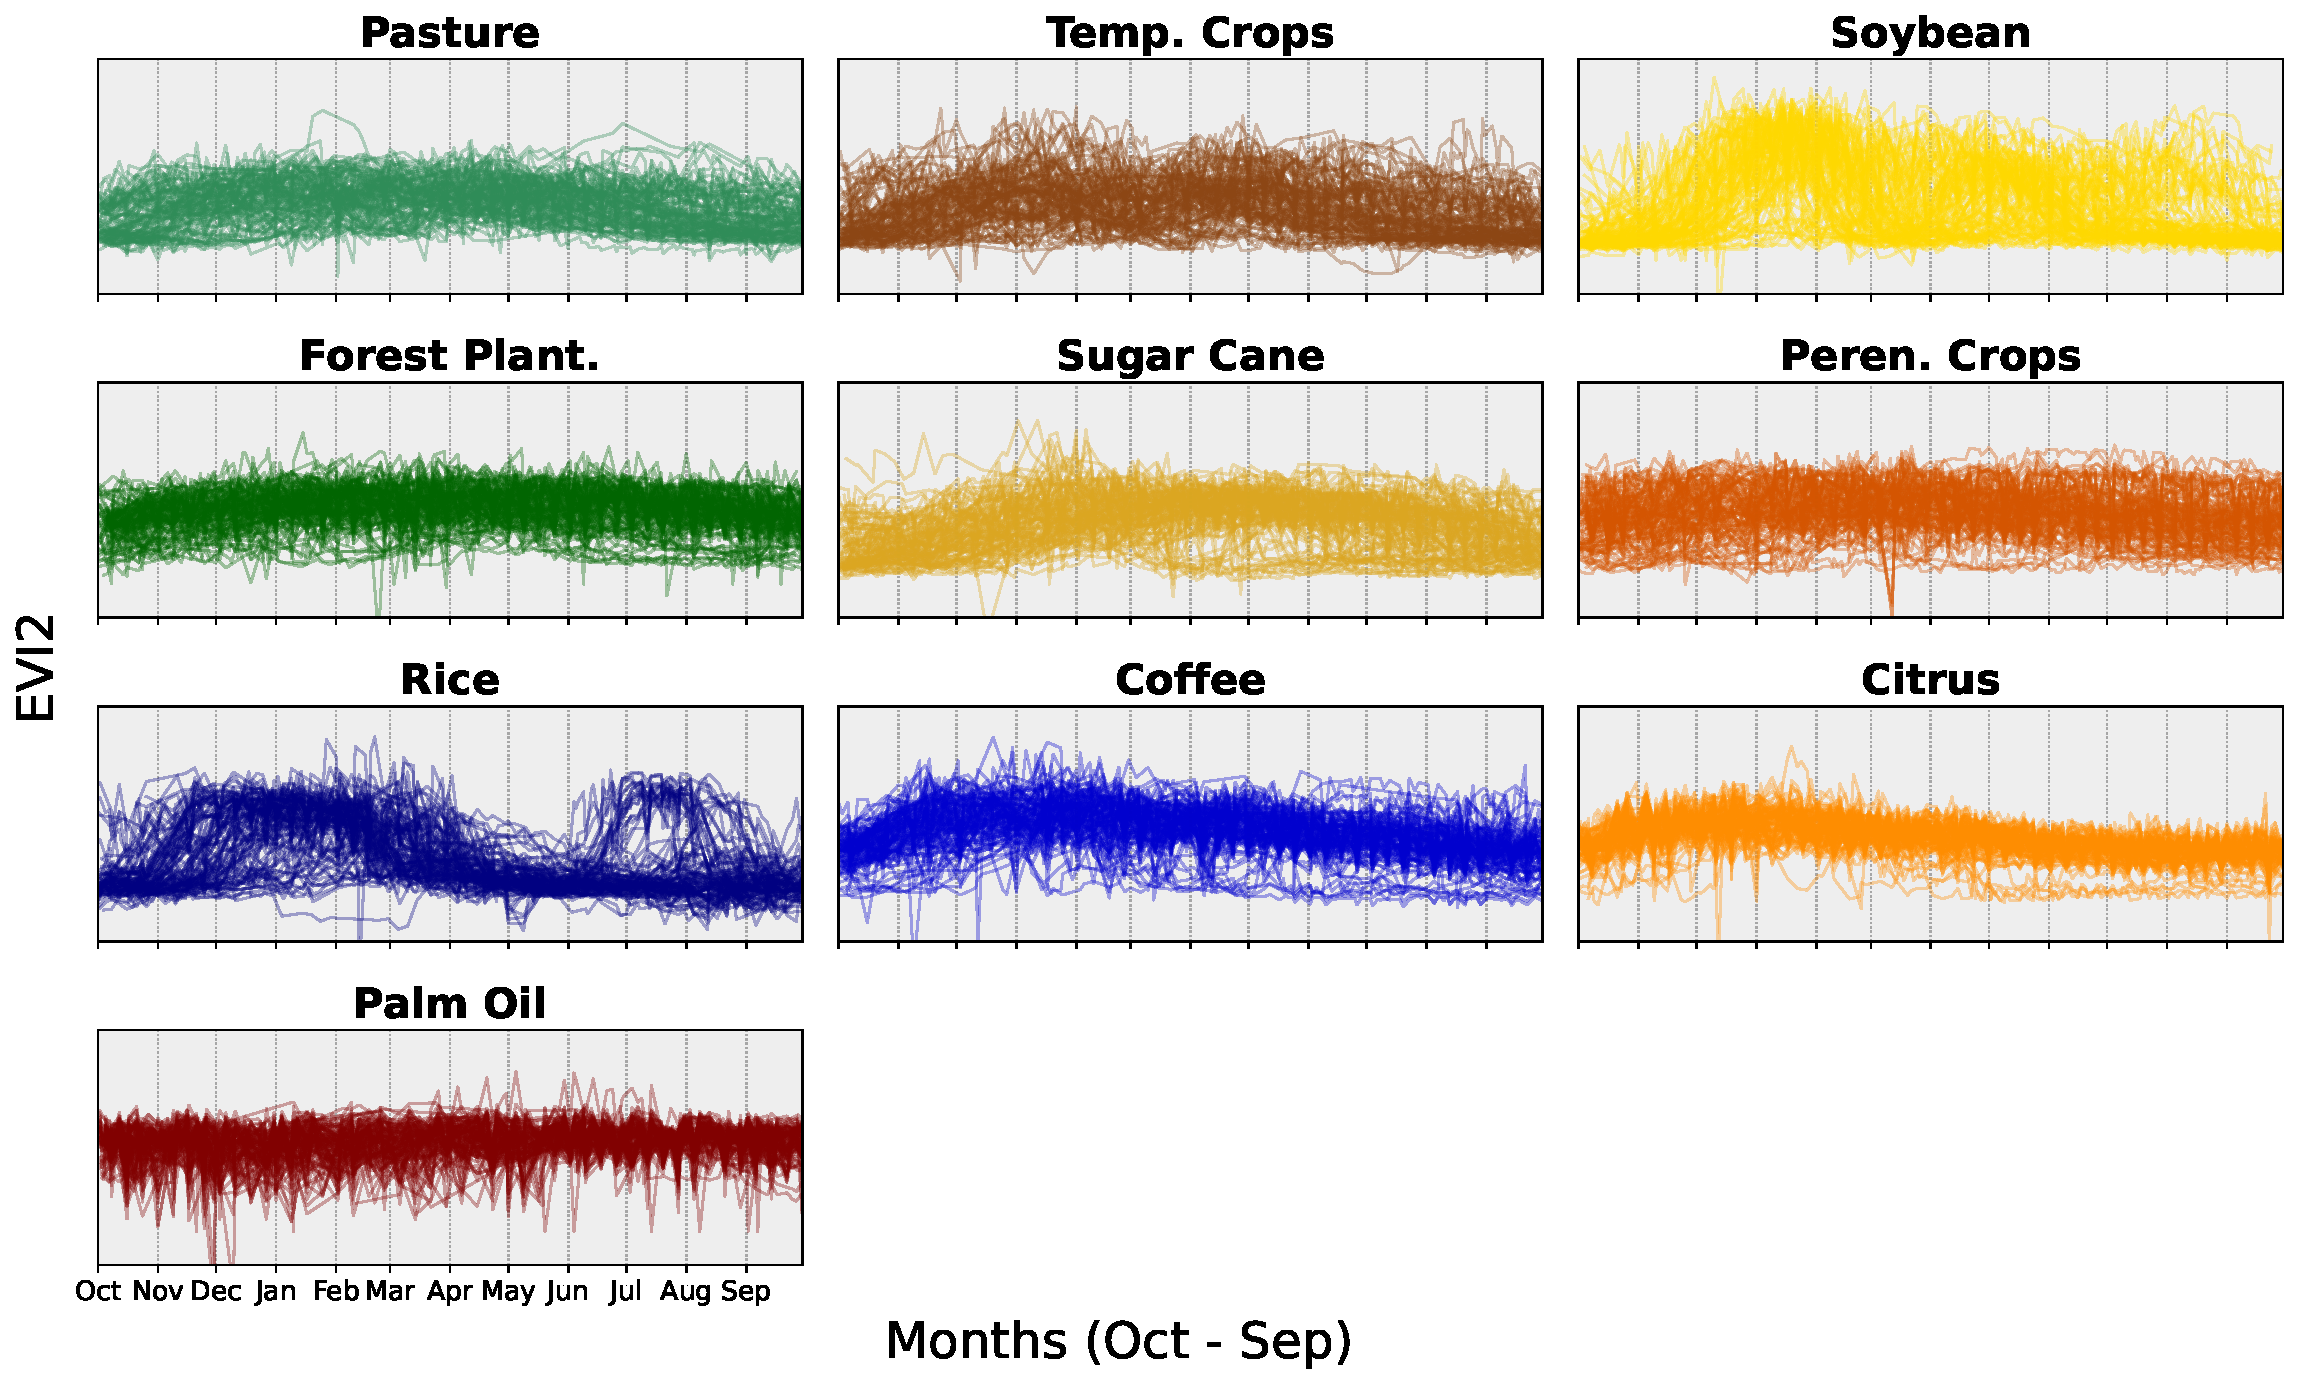
\includegraphics[width=0.7\linewidth]{figures/6_methodology/datasets/brazil_evi2.pdf}
\label{fig:evi2_brazil}
\fignote{Although only EVI2 is shown, which is an agricultural index calculated from Red and NIR and allows for easier visual differentiation of crop classes, the datasets consist of all 10 bands of Sentinel-2.}
\end{figure}

\begin{figure}[ht!]
\centering
\caption{EVI2 per crop class in California SITS dataset.}
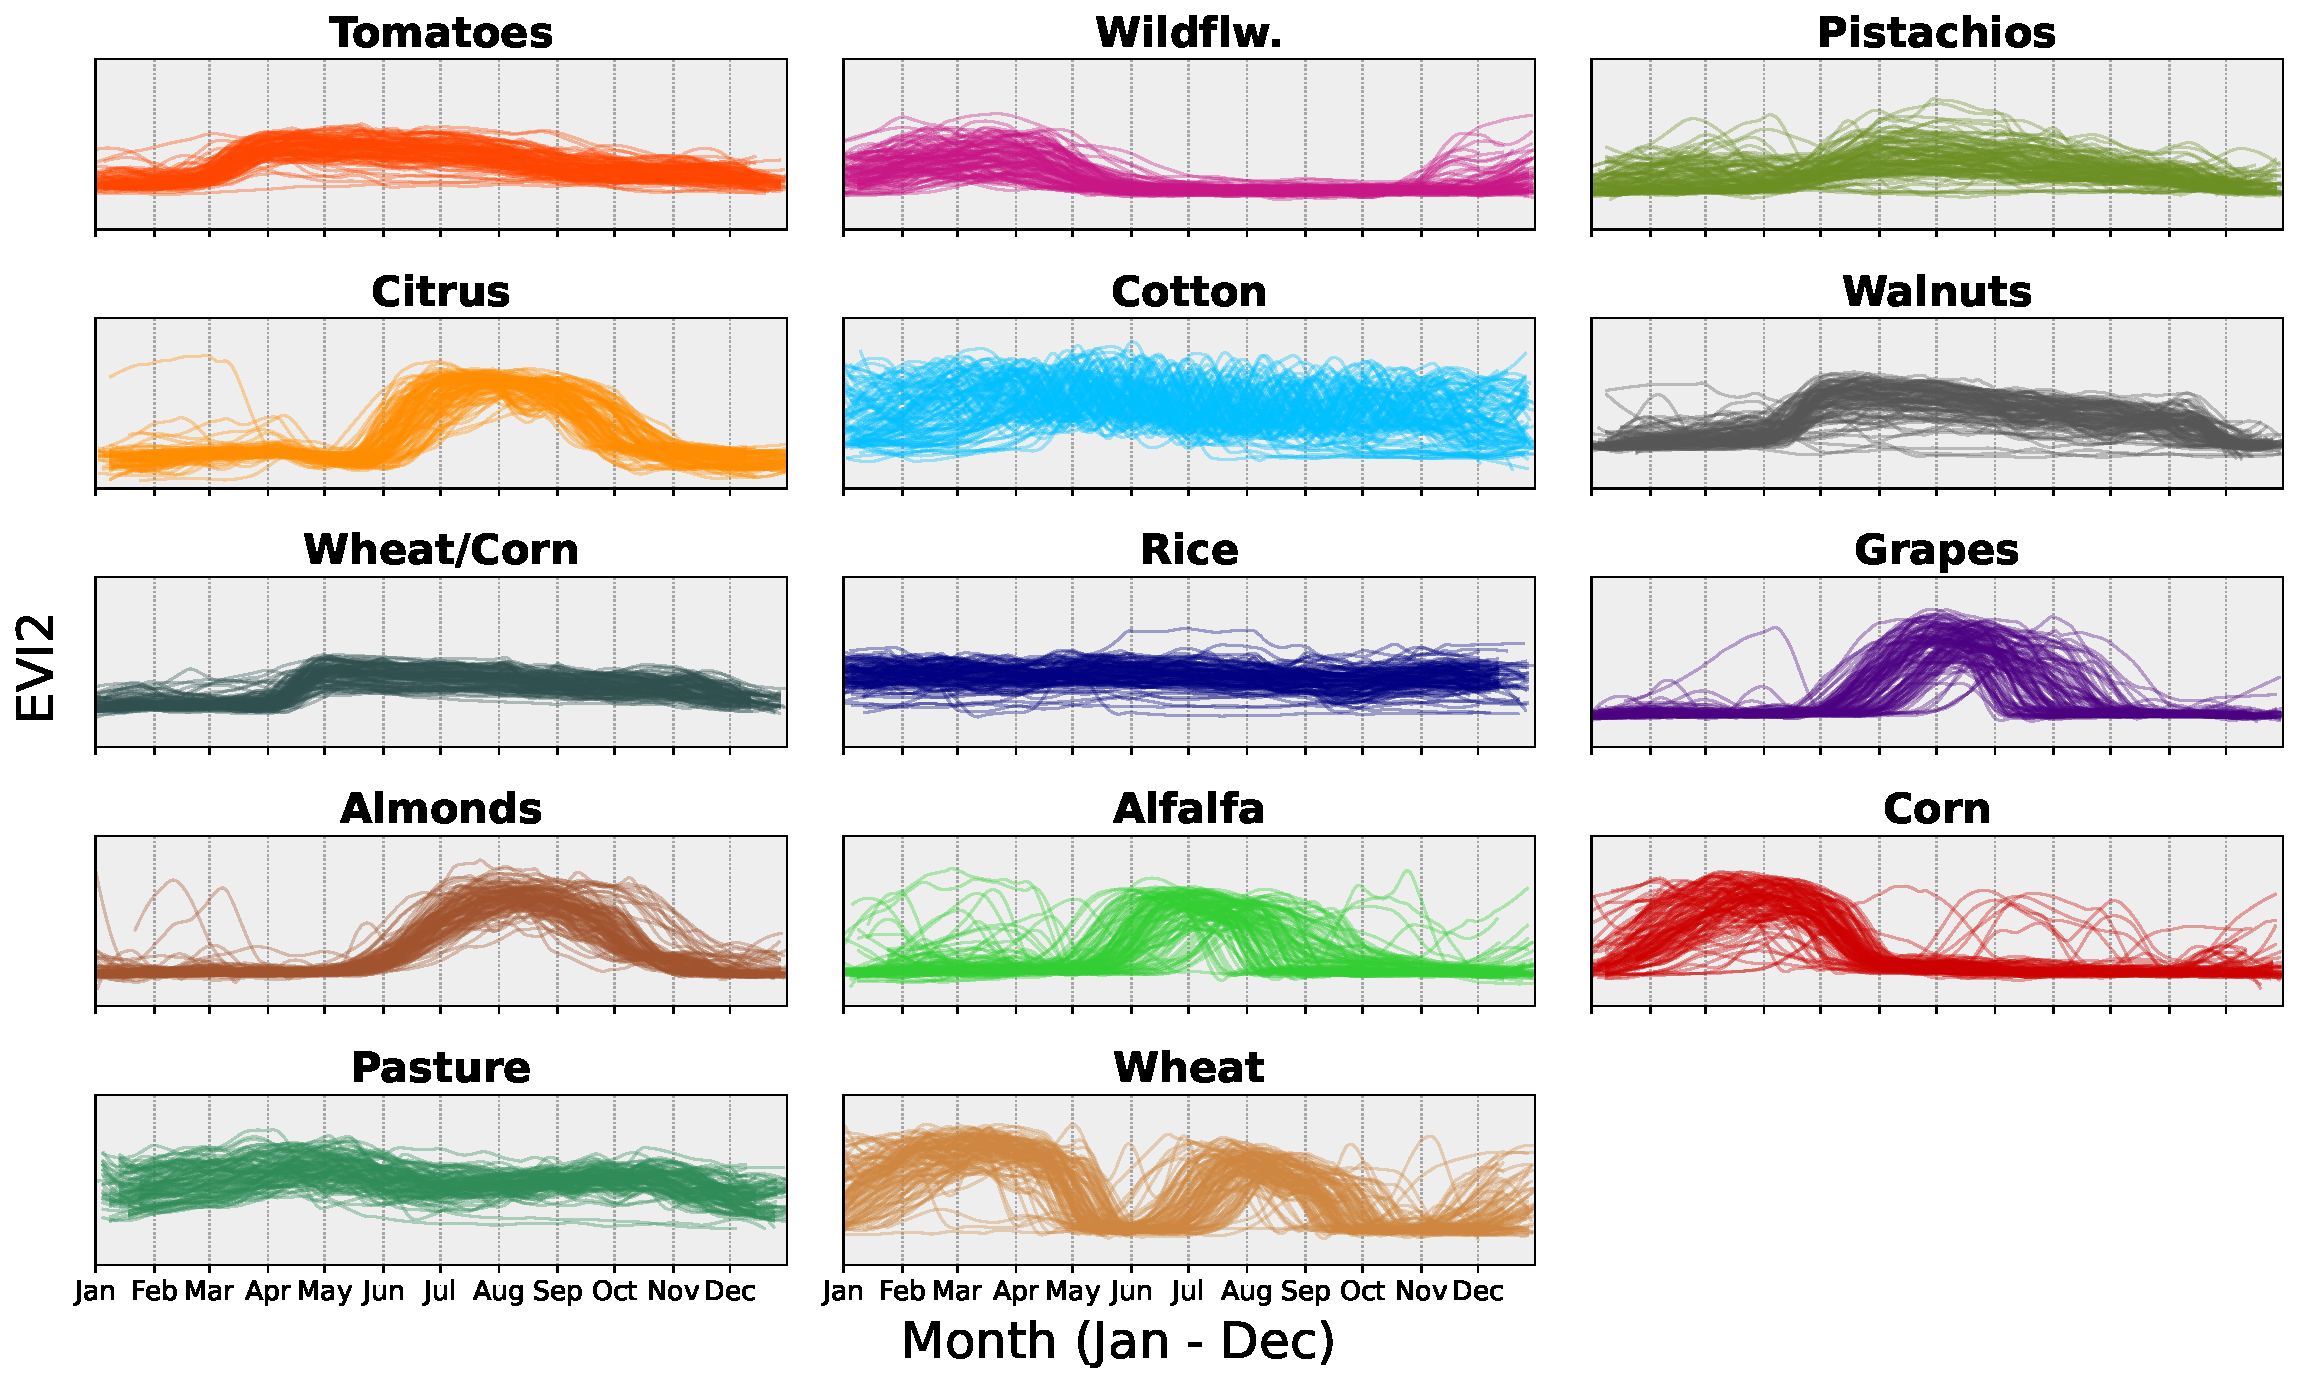
\includegraphics[width=0.7\linewidth]{figures/6_methodology/datasets/california_evi2.pdf}
\label{fig:evi2_california}
\fignote{Although only EVI2 is shown, which is an agricultural index calculated from Red and NIR and allows for easier visual differentiation of crop classes, the datasets consist of all 10 bands of Sentinel-2.}
\end{figure}

\begin{figure}[ht!]
\centering
\caption{EVI2 per crop class in Texas SITS dataset.}
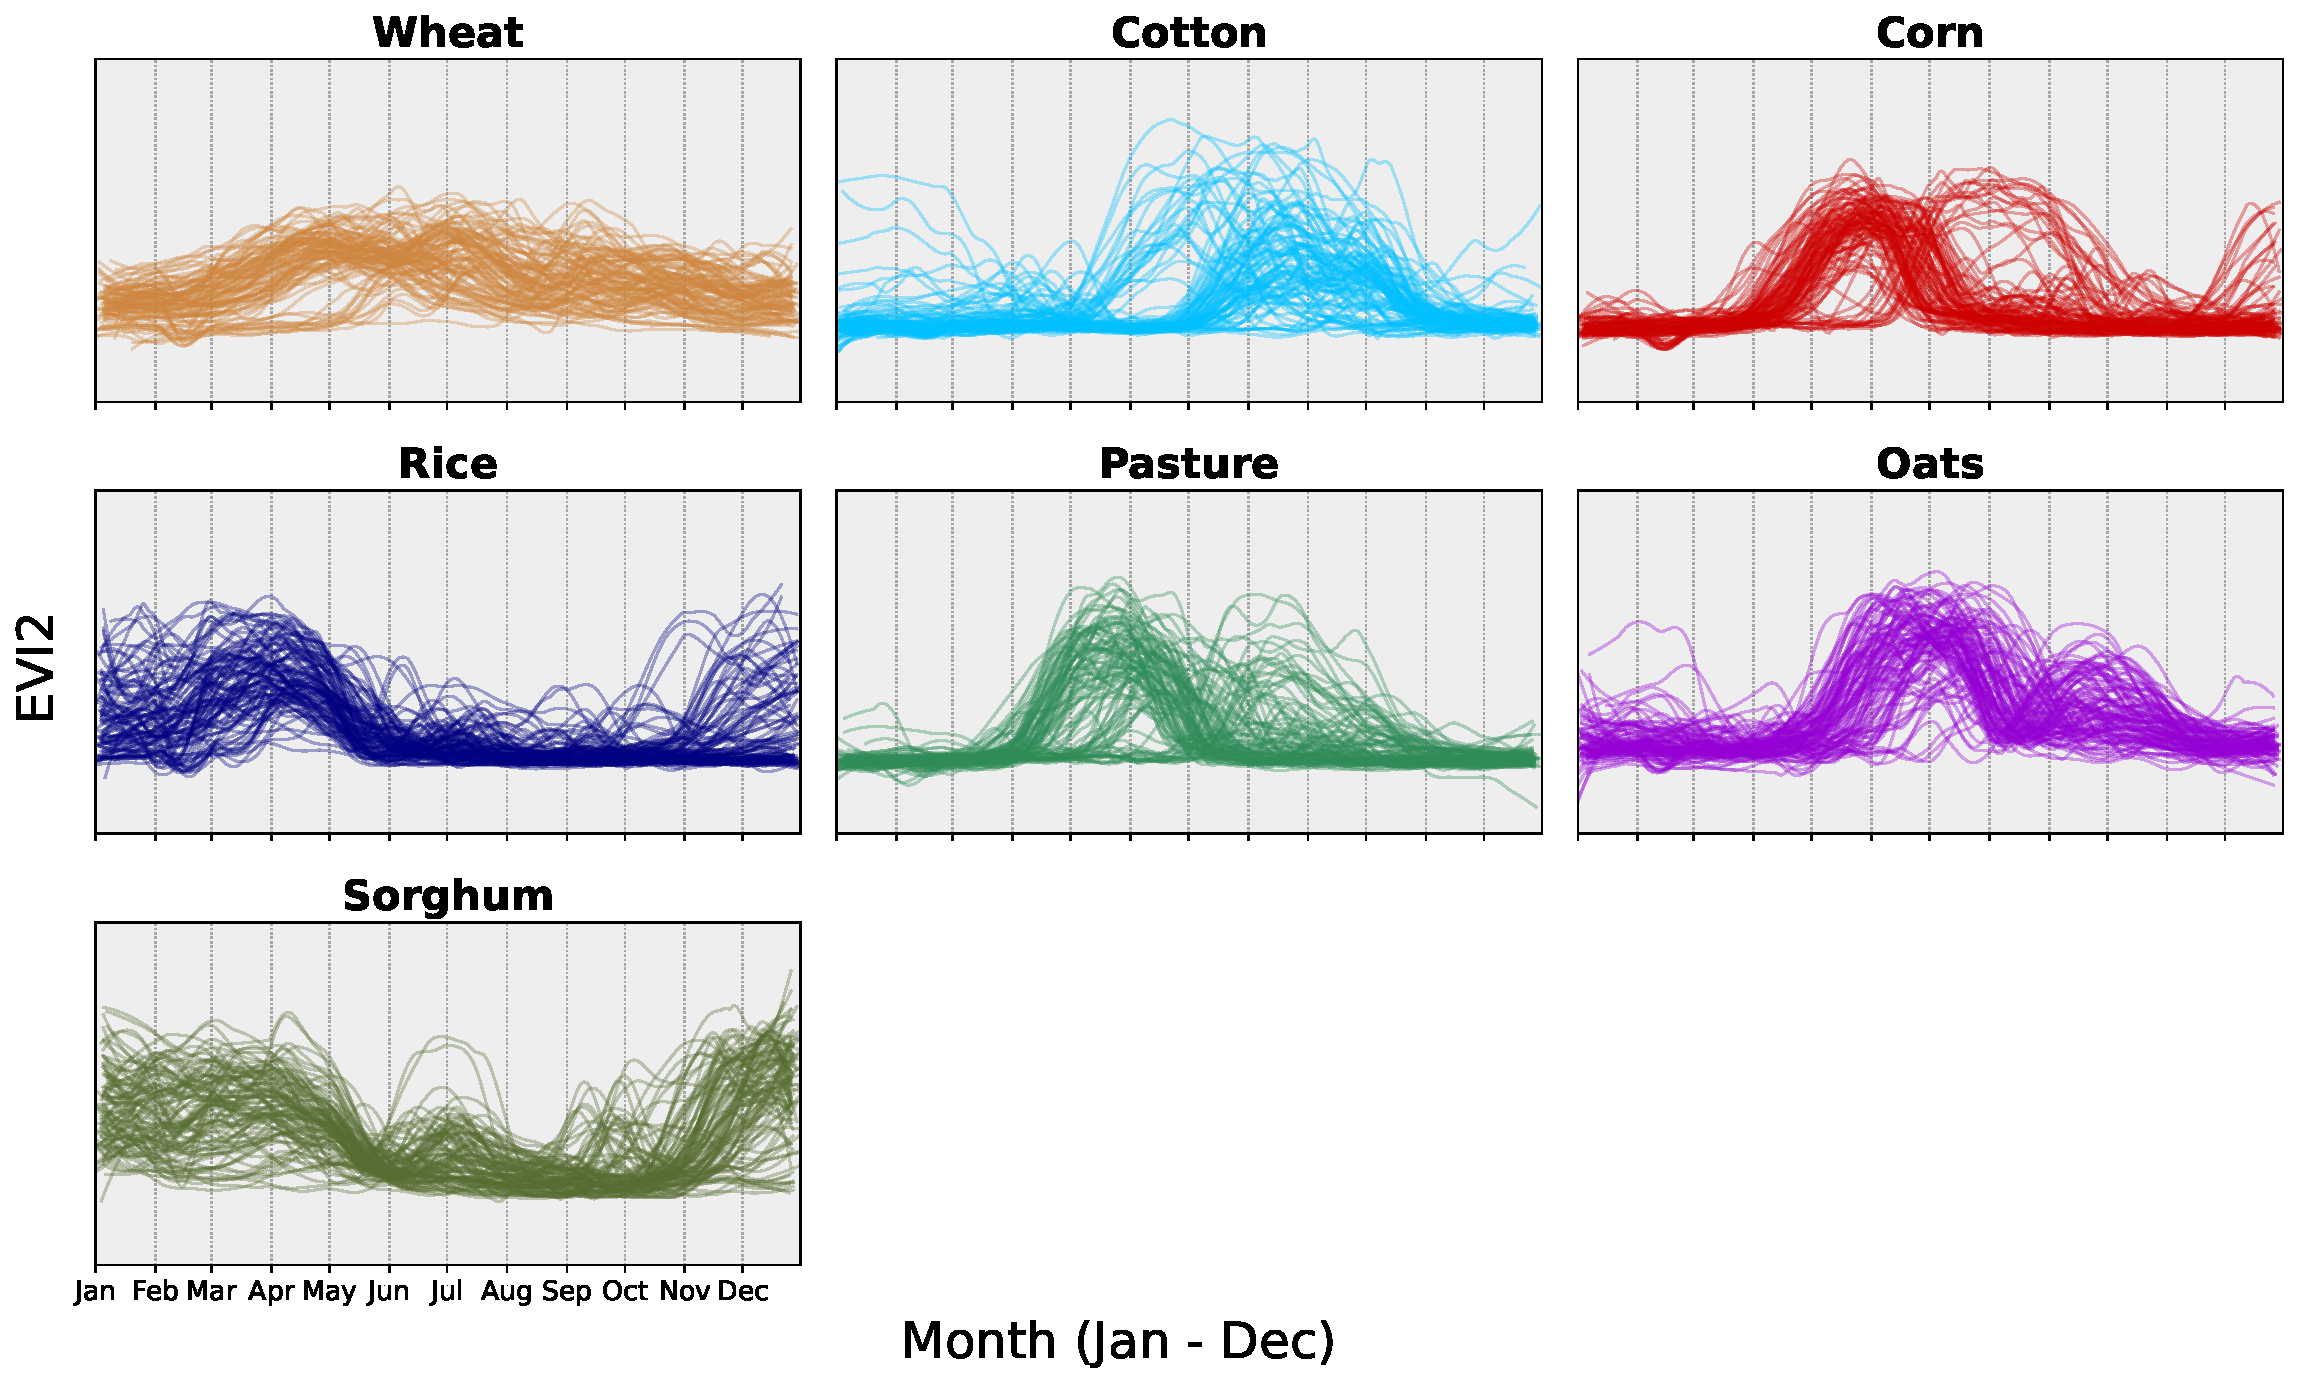
\includegraphics[width=0.7\linewidth]{figures/6_methodology/datasets/texas_evi2.pdf}
\label{fig:evi2_texas}
\fignote{Although only EVI2 is shown, which is an agricultural index calculated from Red and NIR and allows for easier visual differentiation of crop classes, the datasets consist of all 10 bands of Sentinel-2.}
\end{figure}

Finally, the evaluation strategy reflects the varying difficulty of the datasets. A more rigorous division between training, validation, and testing was implemented for Brazil compared to California and Texas. While the US datasets used a stratified split by samples (following \citep{pintodasilva2025lightweight}), the Brazilian dataset was split at the city level. This geographical split prevents spatial leakage and forces the model to generalize to unseen municipalities, making the metrics considerably more realistic and the task more challenging.

\section{The AgriGEE.lite library}
\label{sec:agl}

To facilitate the use of the methodology by other researchers, the lightweight \ac{SITS} download strategy has been coded in our open-source python library AgriGEE.lite. It is a parallel wrapper for \ac{GEE}, designed with the aim of abstracting the complexity of direct programming of the platform and solving performance bottlenecks in \ac{SITS} downloads. By default but optionally, the library abstracts preprocessing steps, such as applying sensor-specific cloud masks, atmospheric corrections, and band harmonization. The library can be installed using PyPI\footnote{PyPI: \url{https://pypi.org/project/agrigee-lite/}} and its source code can be downloaded/checked/reviewed in GitHub\footnote{GitHub: \url{https://github.com/mateuspinto/AgriGEE.lite}}.

The tool's architecture is specifically designed for use with GeoPandas, due to the widespread use of the latter library by remote sensing researchers. The workflow is organized into three main modules: \textbf{agl.sat}, responsible for defining sensors and other data sources; \textbf{agl.vis}, focused on exploratory data visualization; and \textbf{agl.get}, focused on data acquisition, whether parallel or not. One of the technical differences of the library is that downloads are performed by the aria2 utility, allowing the execution of multiple parallel connections outside the Python virtual machine, which enables parallel downloads without dealing with the problems inherent to parallelism and Python's GIL.

Although the methodology of this work specifically uses median statistics applied to Sentinel-2 images to generate the samples, AgriGEE.lite was developed to be agnostic with regard to the sensor and aggregation metric. As detailed in Table \ref{tab:agl_sats}, the library supports a wide range of data sources, including optical sensors (Sentinel-2, Landsat, MODIS), radar sensors (Sentinel-1, PALSAR), Cropland Rasters (MapBiomas, \ac{USDA}), and other products (ANADEM, SoilGrids).

\begin{landscape}
\begin{table}[ht]
\caption{Available data sources of AgriGEE.lite library.}
\centering
\small
\begin{tabular}{|l|p{4cm}|c|c|c|c|c|p{3cm}|}
\hline
\textbf{Name} & \textbf{Bands} & \textbf{Start} & \textbf{End} & \textbf{Region} & \textbf{Pixel size (meters)} & \textbf{Revisit Time} & \textbf{Variations} \\
\hline
Sentinel 2 & VIS, Re1-4, Nir, Swir1-2 & 2016-01-01 & Operational & Global & 10-60 & 5 days & BOA, TOA \\
\hline
Landsat 5 & VIS, Nir, Swir1-2 & 1984-03-01 & 2013-05-05 & Global & 30 & 16 days & - \\
\hline
Landsat 7 & VIS, Nir, Swir1-2, Pan & 1999-04-15 & 2022-04-06 & Global & 15-30 & 16 days & Pan-sharpened \\
\hline
Landsat 8 & VIS, Nir, Swir1-2, Pan & 2013-04-11 & Operational & Global & 15-30 & 16 days & Pan-sharpened \\
\hline
Landsat 9 & VIS, Nir, Swir1-2, Pan & 2021-11-01 & Operational & Global & 15-30 & 16 days & Pan-sharpened \\
\hline
HLS Landsat & Coastal, VIS, Nir, Swir & 2013-04-11 & Operational & Global & 30 & 2-3 days & - \\
\hline
HLS Sent-2 & Coastal, VIS, Re, Nir & 2015-11-30 & Operational & Global & 30 & 2-3 days & - \\
\hline
MODIS & Red, Nir & 2000-02-18 & Operational & Global & 250 & Daily & - \\
\hline
Sentinel 1 & VV, VH (C Band) & 2014-10-03 & Operational & Global & 10 & 5 days & GRD, ARD \\
\hline
JAXA PalSAR & HH, HV (L Band) & 2014-08-04 & Operational & Global & 25 & 15 days & GRD \\
\hline
Sat Embed & 64-dim embedding & 2017-01-01 & 2024-01-01 & Global & 10 & 1 year & - \\
\hline
Mapbiomas & 37 LULC Classes & 1985-01-01 & 2024-12-31 & Brazil & 30 & 1 year & - \\
\hline
ANADEM & Slope, Elevation, Aspect & Single & Single & S. Amer & 30 & Single & - \\
\hline
SoilGrids & WRB Soil Classes & Single & Single & Global & 250 & Single & - \\
\hline
\end{tabular}
\label{tab:agl_sats}
\end{table}
\fignote{The explanation for the abbreviations used in the table is as follows:

\begin{enumerate}
  \item \textbf{BOA -} Bottom of Atmosphere;
  \item \textbf{TOA -} Top of Atmosphere;
  \item \textbf{Pan-sharpened -} Can be downloaded with pan-sharp super resolution applied, increasing spatial resolution to 15 meters;
  \item \textbf{GRD -} Ground Range Detected;
  \item \textbf{ARD -} Analysis Ready Data.
\end{enumerate}
}
\end{landscape}


In addition to flexibility in sensor selection, the tool automates the calculation of spectral indices useful for agricultural and deforestation \ac{RS}, performed in the \ac{GEE} cloud prior to download. The library covers a wide spectrum of optical indices, including those for vegetation health and greenness (e.g., NDVI, EVI, SAVI, GNDVI, NDRE), water content detection (NDWI, MNDWI), and soil characteristics (BSI). Furthermore, specific indices for Synthetic Aperture Radar (SAR) data are implemented, such as the Radar Vegetation Index (RVI) and polarization ratios (VH/VV, HH/HV).

Similarly, for scenarios that require statistics other than the median, the library offers several spatial reducers allowing use in various experimental setups. The available statistics encompass measures of central tendency (mean, mode), dispersion (standard deviation, variance, minimum, maximum), and distribution shape (kurtosis, skewness). Users can also request arbitrary percentiles to capture specific segments of the data distribution.